\documentclass[10pt,a4paper]{article}
\usepackage[T1]{fontenc}
\usepackage[utf8]{inputenc}
\usepackage{lmodern}
\usepackage{textcomp}
\usepackage[margin=2.2cm]{geometry}
\usepackage{microtype}
\usepackage{graphicx}
\usepackage{booktabs}
\usepackage{longtable}
\usepackage{tabularx}
\usepackage{adjustbox}
\usepackage{fancyvrb}
\usepackage{enumitem}
\usepackage{xcolor}
\usepackage{newunicodechar}
\usepackage[hidelinks]{hyperref}
\setlist{itemsep=2pt,topsep=3pt}
\setlength{\parskip}{4pt}
\setlength{\parindent}{0pt}
\setlength{\emergencystretch}{3em}
\renewcommand{\arraystretch}{1.1}
\newunicodechar{∪}{\ensuremath{\cup}}
\newunicodechar{→}{\ensuremath{\to}}
\newunicodechar{≥}{\ensuremath{\geq}}
\newunicodechar{≤}{\ensuremath{\leq}}
\newunicodechar{−}{\ensuremath{-}}
\newunicodechar{≈}{\ensuremath{\approx}}
\newunicodechar{±}{\ensuremath{\pm}}
\newunicodechar{×}{\ensuremath{\times}}
\newunicodechar{·}{\ensuremath{\cdot}}
\newunicodechar{Σ}{\ensuremath{\Sigma}}
\newunicodechar{⁻}{\ensuremath{^{-}}}
\newunicodechar{⁰}{\ensuremath{^{0}}}
\newunicodechar{²}{\ensuremath{^{2}}}
\newunicodechar{⁵}{\ensuremath{^{5}}}
\newunicodechar{⁶}{\ensuremath{^{6}}}
\newcommand{\code}[1]{\texttt{#1}}
\newcommand{\tablecaption}[1]{\par\smallskip\noindent{\small #1}\par\nopagebreak}
\newcommand{\tablenote}[1]{\par\noindent{\footnotesize #1}\par\medskip}
\title{Learned Page Replacement for xv6 — Study on the \code{traces2} Streams}
\date{}
\begin{document}
\maketitle
\vspace{-2em}
\textbf{Status:} complete study on the verified seed/variant streams (\code{traces2/\allowbreak{}}). Supersedes the numbers in \code{report/\allowbreak{}ML\_\allowbreak{}TESTING\_\allowbreak{}REPORT.\allowbreak{}md}, which was measured on the older \code{traces/\allowbreak{}} captures — two of which turned out to be wrong (§2.4). That report is kept for history; nothing in this one depends on it.

\section*{Summary}
\addcontentsline{toc}{section}{Summary}

\textbf{Question.} Can a learned model replace the page-replacement policy of an operating system — first in xv6-riscv, eventually in Linux?

\textbf{Data.} 89 verified reference streams (123M references) from five native xv6 workloads in 25 variants, every access marked read or write, with fixed train / validation / test (unseen seeds) / held-out (unseen variants) splits and Belady-optimal labels (§2–3).

\textbf{What was tried.} Twelve per-page features in three tiers — \emph{oracle} features a kernel can never see (exact recency, frequency, stack distance, write ratio), \emph{kernel-observable} features from accessed/dirty-bit scans, and \emph{refault} bookkeeping Linux already keeps — and \textbf{every combination}: 300 feature sets × 6 training scopes as linear models (28,800 full replays), plus MLPs, ranking-loss models, a GRU over each page's access history, and a cross-page embedding model (§4–5). Models are selected on validation only.

\textbf{Results.}

\begin{enumerate}
\item \textbf{A linear score over 4–5 kernel-observable features beats xv6's best built-in policy (Clock) on all five workloads, on unseen seeds and on unseen variants}: btree −17\% faults (test) / −14\% (held-out), graph −15\% / −20\%, kv −10\% / −10\%, matmul −32\% (held-out), sort −2\% / −7\% (§6.5). It needs up to \textbf{66\% fewer disk writes} (graph), because it uses the dirty bit (§6.6).
\item \textbf{Oracle information buys almost nothing} over the kernel's own signals: the best full-stream model is within ±1.5\% on btree, graph and kv and behind on matmul and sort. The single most valuable feature is \code{idle} — scans since the page was last found accessed, which Linux's MGLRU and DAMON already track (§6.4, §9).
\item \textbf{Bigger models do not pay.} MLPs help on kv (4–6\%) and held-out graph, not consistently elsewhere; the GRU adds nothing; the cross-page embedding is catastrophic on btree and graph (and best on held-out kv); a ranking loss is worse than regression (§6.7).
\item \textbf{It runs without floating point.} Integer-only scoring with 8-bit weights is within ±0.002 of the float result everywhere (§8).
\item \textbf{The failure modes are real and were found and fixed.} Many feature sets are catastrophic (≥3× Clock), and the first training set taught models to evict the page being streamed through — diagnosed from the policies' own decisions and fixed by recency-stratified recording and a probation for new pages, both chosen on validation (§7).
\item \textbf{It works inside xv6.} The model runs as \code{VM\_\allowbreak{}POLICY\_\allowbreak{}ML} in the kernel (integer-only, weights per process via \code{vmctl}). It passes the data-invariance suite, and in 231 in-kernel runs at 10\% memory it beats Clock on every workload, on unseen seeds and on unseen variants: btree −18\% / −15\% faults (test / held-out), graph −39\% / −46\%, kv −13\% / −13\%, sort −4\% / −7\%, matmul −3\% (held-out). Page writes drop by up to 96\%. The simulator predicted these runs closely, except one PageRank stream that sits on a capacity cliff. The price is victim selection, at 11–13× Clock's cost per eviction (§8b).
\item \textbf{Limitations.} Graph's gain in the simulator is concentrated at 10\% of its pages (§6.5), and the in-kernel runs cover only 10\%. One global model keeps most of the gain on btree/graph/kv but loses to Clock on matmul, in the kernel too. Selection scans the whole resident set (§10).
\end{enumerate}

\textbf{Corrections to the earlier report.} Its graphbench and lzwbench results were measured on broken traces (§2.4); its ``stack distance'' was not stack distance (§4). Neither should be cited.

\clearpage\tableofcontents\clearpage
\section*{1. Question and constraints}
\addcontentsline{toc}{section}{1. Question and constraints}

The research question: \textbf{can a learned model replace the classical page-replacement policy of an operating system?} The plan is to show it in xv6-riscv first — train on memory workloads, integrate the model into the kernel, measure it — as a precursor to doing the same in Linux.

Three constraints shape every design decision below.

\begin{enumerate}
\item \textbf{xv6 has no floating point.} Nothing learned can run in the kernel unless it can be computed in integers. All training here runs on the host (Python/PyTorch); the question of what could run \emph{inside} the kernel is answered separately (§8).
\item \textbf{A kernel does not see memory accesses.} A load or store is handled entirely by the MMU. What the kernel sees is (a) page faults and (b) the accessed (\code{PTE\_\allowbreak{}A}) and dirty (\code{PTE\_\allowbreak{}D}) bits the hardware sets in the page table, which the kernel can read and clear when it scans pages. This is equally true of Linux for anonymous memory. So a model that needs ``how many times was this page touched'' or ``how long since its last access, in accesses'' cannot be deployed as trained; it needs information the kernel never has. This study therefore trains every model on three feature tiers (§4) — what only an oracle trace has, what a kernel can observe, and what a kernel can cheaply book-keep — and treats the first as an ablation (an upper bound on what information is worth), not as a deployable result.
\item \textbf{Decisions compound.} Which page is evicted changes every later fault, so policies can only be compared by replaying complete reference streams, never by per-reference prediction accuracy. All results are fault counts from full replays.
\end{enumerate}

\section*{2. How the traces were made}
\addcontentsline{toc}{section}{2. How the traces were made}

\subsection*{2.1 The workloads}
\addcontentsline{toc}{subsection}{2.1 The workloads}

Five native xv6 programs (\code{user/\allowbreak{}*bench.\allowbreak{}c}), each built so that no single fixed heuristic — pure recency, pure frequency, pure sequential — wins trivially (\code{docs/\allowbreak{}workloads.\allowbreak{}md}):

\begin{center}\footnotesize
\begin{tabularx}{\linewidth}{lXX}
\toprule
\textbf{Workload} & \textbf{What it models} & \textbf{Why it isn't trivial for one policy} \\ \midrule
\code{btreebench} & A B+tree over 4 KB node pages (SQLite pager stand-in): insert, point lookup, range scan, mixed; optional write-ahead log & Lookups re-hit the same upper nodes (frequency), inserts touch fresh leaves once (recency), scans walk the leaf chain (sequential) \\
\code{kvbench} & An open-addressing hash table with Zipfian keys (Redis stand-in), YCSB-style modes A (50/50 r/w), B (95/5), C (read-only), D (read-latest), F (read-modify-write); optional incremental rehash and heavy-tailed value sizes & The hot key set rotates over time, so old-hot pages must go cold and new-hot ones warm up \\
\code{graphbench} & BFS and fixed-point PageRank over a synthetic scale-free graph (CSR layout) & BFS visits pages in data-dependent frontier order; PageRank revisits hub vertices every iteration \\
\code{sortbench} & Bottom-up merge sort & Deliberately sequential — a calibration workload with little headroom \\
\code{matmulbench} & Integer matrix multiply, naive (ijk) vs. blocked & A locality-contrast pair; tiny working sets \\
\bottomrule
\end{tabularx}
\end{center}

\subsection*{2.2 What a trace records}
\addcontentsline{toc}{subsection}{2.2 What a trace records}

Each workload routes every access to its data arena through one accessor (e.g. \code{bt\_\allowbreak{}node()}, \code{graph\_\allowbreak{}trace()}), which calls \code{vmbench\_\allowbreak{}trace\_\allowbreak{}ref(vpn,\allowbreak{} access)} and emits one line per logical access: \code{R <vpn>} if the access only read the page, \code{W <vpn>} if it modified it. The access argument has no default, so an untraced or unmarked call site does not compile. The stream is a \textbf{complete reference string} — every touch, not just faults — which is what an optimal (Belady) label needs: a page that stays resident and is re-touched without faulting is still recorded. Only the arena is traced; the process's own code and stack pages (3–9 always-hot frames per run) are not.

The trace is written to a file inside xv6's file system (one \code{write()} per \textasciitilde{}4 KB, rather than a character at a time over the console) and extracted on the host afterwards.

\subsection*{2.3 How the stream set was collected (AU5TRA, commits \code{2d89a64}–\code{e6bfafe})}
\addcontentsline{toc}{subsection}{2.3 How the stream set was collected (AU5TRA, commits \code{2d89a64}–\code{e6bfafe})}

A reference string does not depend on how much memory the run is given — verified: every capacity of a workload in the older \code{traces/\allowbreak{}sweep} campaign produced a byte-identical trace. So each stream needs \textbf{one traced run at a generous margin} (8,000 resident frames, above every footprint), not a capacity sweep; capacities are then chosen in simulation.

\begin{itemize}
\item \code{tools/\allowbreak{}make\_\allowbreak{}stream\_\allowbreak{}manifest.\allowbreak{}py} defines the matrix: 25 variants — kv ×7, btree ×5, graph ×4, sort ×3, matmul ×6 — and seeds per variant (5, or 3 for the long graph and sort runs; matmul's seed only fills in matrix values, so it has one stream per variant). \textbf{89 streams}, plus 22 \code{-rep} determinism repeats.
\item \code{tools/\allowbreak{}run\_\allowbreak{}stream\_\allowbreak{}lanes.\allowbreak{}sh} runs them in 6 parallel lanes, each in its own copy of the tree; every run gets a freshly built \code{fs.\allowbreak{}img}.
\item A stream counts as collected only if the run printed PASS, the log carries \code{TRACEEND refs=N bytes=M}, and the extracted file has exactly N lines and M bytes, every one \code{R <vpn>} or \code{W <vpn>}.
\item \code{tools/\allowbreak{}check\_\allowbreak{}streams.\allowbreak{}py} then checks that every repeat is byte-identical to its original, every trace is under 90\% of xv6's maximum file size, and the seeds of a variant give different strings.
\end{itemize}

All 111 runs passed; all 22 repeats were byte-identical. Deliberately left out: kvbench's TTL mode (expiry reads \code{uptime()}, so the string depends on timing), lzwbench (its string exceeds xv6's maximum file size), and matmul seeds (no effect).

\subsection*{2.4 Why the older \code{traces/\allowbreak{}} captures are not used}
\addcontentsline{toc}{subsection}{2.4 Why the older \code{traces/\allowbreak{}} captures are not used}

Checking the dataset against the kernel's own counters and against host re-executions of the workloads (commit \code{9d36525}) found two of the six old captures wrong:

\begin{itemize}
\item \textbf{graphbench} traced only the edge array. BFS's \code{visited[]} checks and PageRank's \code{rank[]}/\code{next\_\allowbreak{}rank[]} updates — the random, hub-driven accesses the workload exists for — were never recorded: 667 of 2,000 arena pages and 57\% of the references. FIFO over the old trace could not reproduce the kernel's eviction count (168,551 vs. 2,035,488).
\item \textbf{lzwbench}'s trace hit xv6's maximum file size (67,381,296 of 67,382,272 bytes) and silently lost its tail — about 58\% of the run is present — while the run still printed PASS.
\end{itemize}

The other four old traces are page-for-page identical to their \code{traces2} counterparts (btree-mixed-s1, kv-A-s1, sort-n40000-s1, matmul-*96), just without read/write marks. Consequences for the earlier report: its graphbench result (``\code{global\_\allowbreak{}frequency} beats Clock by 4.3\%'') and its lzwbench result (``hand-written LFU −24\% vs. Clock'') were measured on these two broken traces and should not be cited. With the fixes, the new graph traces match a host re-execution reference for reference, FIFO over them reproduces the kernel's evictions with 3–5 untraced frames (−0.1\%), and a dirty-tracking replay of the W marks predicts the kernel's own \code{page\_\allowbreak{}writes} (btree 12,329 inside [12,168, 12,438]).

\code{traces/\allowbreak{}} is still used for what it is good at — its \code{sweep/\allowbreak{}} campaign holds real kernel fault counts at six resident limits per workload, which is how the simulator's agreement with the kernel is established — but not for ML.

\section*{3. The dataset (\code{traces2/\allowbreak{}ML})}
\addcontentsline{toc}{section}{3. The dataset (\code{traces2/\allowbreak{}ML})}

\code{tools/\allowbreak{}stream\_\allowbreak{}dataset.\allowbreak{}py prepare} turns the 89 streams into:

\begin{itemize}
\item \code{<stem>.\allowbreak{}npz} — three aligned arrays, one entry per reference: \code{vpn} (uint32), \code{write} (bool), and \code{next\_\allowbreak{}use} — the distance, in references, to the next access of the same page (\code{0xFFFFFFFF} if never). \code{next\_\allowbreak{}use} is the quantity Belady's algorithm evicts by; it is computed from the recorded future and is used \textbf{only as a training label and for the Belady baseline, never as a model input}.
\item \code{SPLITS.\allowbreak{}tsv} — fixed splits, so every experiment reports against the same data:

\begin{itemize}
\item \textbf{held-out}: whole variants never seen in training — \code{kv-F}, \code{btree-scan}, \code{graph-bfs2000}, \code{sort-n60000}, \code{matmul-*128}. This tests an unseen \emph{behaviour}.
\item within every other variant: last seed \textbf{test}, second-to-last \textbf{validation}, the rest \textbf{train}. This tests an unseen \emph{run} of a familiar behaviour.
\end{itemize}
\item \code{baselines.\allowbreak{}tsv} — FIFO, LRU and Belady fault counts at six capacities (5, 10, 15, 20, 25, 30\% of the stream's own distinct pages), simulated from empty memory.
\end{itemize}

\begin{center}\footnotesize
\begin{adjustbox}{max width=\linewidth}
\begin{tabular}{lrl}
\toprule
\textbf{Split} & \textbf{Streams} & \textbf{References} \\ \midrule
train & 41 & 45.5M \\
val & 15 & 23.6M \\
test & 15 & 23.6M \\
held-out & 18 & 30.6M \\
\bottomrule
\end{tabular}
\end{adjustbox}
\end{center}

Per variant (means over its streams):

\begin{center}\footnotesize
\begin{adjustbox}{max width=\linewidth}
\begin{tabular}{llrlrrr}
\toprule
\textbf{Workload} & \textbf{Variant} & \textbf{Streams} & \textbf{Splits} & \textbf{References} & \textbf{Distinct pages} & \textbf{Write share} \\ \midrule
btree & \code{btree-insert} & 5 & train:3, val:1, test:1 & 210,146 & 4,107 & 0.27 \\
btree & \code{btree-lookup} & 5 & train:3, val:1, test:1 & 328,417 & 2,182 & 0.09 \\
btree & \code{btree-mixed} & 5 & train:3, val:1, test:1 & 223,358 & 1,760 & 0.10 \\
btree & \code{btree-mixedwal} & 5 & train:3, val:1, test:1 & 241,295 & 1,761 & 0.17 \\
btree & \code{btree-scan} & 5 & heldout:5 & 412,599 & 2,182 & 0.07 \\
graph & \code{graph-bfs2000} & 3 & heldout:3 & 3,183,375 & 1,665 & 0.16 \\
graph & \code{graph-both1000x3} & 3 & train:1, val:1, test:1 & 6,200,054 & 999 & 0.41 \\
graph & \code{graph-both2000x1} & 5 & train:3, val:1, test:1 & 6,255,588 & 1,997 & 0.33 \\
graph & \code{graph-pr2000x2} & 3 & train:1, val:1, test:1 & 6,143,976 & 1,667 & 0.50 \\
kv & \code{kv-A} & 5 & train:3, val:1, test:1 & 160,326 & 528 & 0.44 \\
kv & \code{kv-Arehash} & 5 & train:3, val:1, test:1 & 478,839 & 749 & 0.40 \\
kv & \code{kv-Avsize} & 5 & train:3, val:1, test:1 & 318,146 & 672 & 0.22 \\
kv & \code{kv-B} & 5 & train:3, val:1, test:1 & 106,211 & 528 & 0.24 \\
kv & \code{kv-C} & 5 & train:3, val:1, test:1 & 100,152 & 527 & 0.20 \\
kv & \code{kv-D} & 5 & train:3, val:1, test:1 & 106,099 & 528 & 0.24 \\
kv & \code{kv-F} & 5 & heldout:5 & 320,626 & 528 & 0.44 \\
matmul & \code{matmul-blocked128} & 1 & heldout:1 & 4,734,976 & 48 & 0.06 \\
matmul & \code{matmul-blocked64} & 1 & train:1 & 593,920 & 12 & 0.06 \\
matmul & \code{matmul-blocked96} & 1 & train:1 & 1,999,872 & 27 & 0.06 \\
matmul & \code{matmul-naive128} & 1 & heldout:1 & 4,210,688 & 48 & 0.00 \\
matmul & \code{matmul-naive64} & 1 & train:1 & 528,384 & 12 & 0.01 \\
matmul & \code{matmul-naive96} & 1 & train:1 & 1,778,688 & 27 & 0.01 \\
sort & \code{sort-n20000} & 3 & train:1, val:1, test:1 & 867,311 & 40 & 0.35 \\
sort & \code{sort-n40000} & 3 & train:1, val:1, test:1 & 1,854,631 & 79 & 0.34 \\
sort & \code{sort-n60000} & 3 & heldout:3 & 2,800,589 & 118 & 0.34 \\
\bottomrule
\end{tabular}
\end{adjustbox}
\end{center}

\section*{4. Features}
\addcontentsline{toc}{section}{4. Features}

Every learned policy scores each resident page at each eviction and evicts the one with the highest predicted next-use distance. Twelve per-page features are available, in three tiers.

\textbf{F — full-stream (oracle; not observable by any kernel).} Need every access.

\begin{center}\footnotesize
\begin{adjustbox}{max width=\linewidth}
\begin{tabular}{ll}
\toprule
\textbf{Feature} & \textbf{Definition} \\ \midrule
\code{rec} & references since the page's last access \\
\code{freq} & exact number of accesses so far \\
\code{sd} & stack distance: \emph{distinct} pages accessed since its last access \\
\code{wr} & fraction of its accesses that were writes \\
\bottomrule
\end{tabular}
\end{adjustbox}
\end{center}

\textbf{K — kernel-observable.} What a kernel can compute from the accessed and dirty bits when it scans the resident pages at an eviction — exactly what xv6's \code{sample\_\allowbreak{}page()}/\code{choose\_\allowbreak{}aging()} already do. Time is counted in scans (one per eviction).

\begin{center}\footnotesize
\begin{tabularx}{\linewidth}{lXX}
\toprule
\textbf{Feature} & \textbf{Definition} & \textbf{Linux analogue} \\ \midrule
\code{ref} & accessed bit at this scan & \code{PG\_\allowbreak{}referenced} / young bit \\
\code{aging} & 8-bit aging counter (shift right, set top bit if accessed) — xv6's Aging state & — \\
\code{sfreq} & number of scans that found it accessed since it was loaded & DAMON \code{nr\_\allowbreak{}accesses}, MGLRU tiers \\
\code{idle} & scans since it was last found accessed & MGLRU generation age, DAMON age \\
\code{age} & scans since it was loaded & — \\
\code{dirty} & dirty bit & \code{PG\_\allowbreak{}dirty} \\
\bottomrule
\end{tabularx}
\end{center}

\textbf{K+ — cheap kernel bookkeeping Linux already does.} Linux's \code{mm/\allowbreak{}workingset.\allowbreak{}c} leaves a small ``shadow'' entry when it evicts a page and, on refault, measures how many evictions happened in between. xv6 already keeps per-page swap-slot metadata, so the same is a few bytes per page.

\begin{center}\footnotesize
\begin{adjustbox}{max width=\linewidth}
\begin{tabular}{ll}
\toprule
\textbf{Feature} & \textbf{Definition} \\ \midrule
\code{refaults} & times this page was evicted and faulted back in \\
\code{rdist} & evictions between its last eviction and its refault \\
\bottomrule
\end{tabular}
\end{adjustbox}
\end{center}

All counts enter as \code{log1p(count)}; every feature is standardised with the training scope's mean and standard deviation.

\textbf{Two things the earlier study got wrong about features}, found while building this one:

\begin{itemize}
\item \emph{Its ``stack distance'' was not stack distance.} \code{tools/\allowbreak{}sim.\allowbreak{}py}'s \code{StackDistance} and the old feature code counted pages touched for the \textbf{first time ever} since a page's last access, not distinct pages. The true stack distance of a resident page orders the resident set exactly like recency, so a linear scorer on \code{sd} alone reproduces LRU's fault count exactly — checked (\code{kv-A-s5}: 10,185 = 10,185). The old policy is kept here as \code{sd\_\allowbreak{}old} for the record.
\item \emph{Pooled correlation misleads.} What matters is whether a feature ranks the candidates of one eviction decision correctly. §6.2 reports both.
\end{itemize}

\section*{5. Method}
\addcontentsline{toc}{section}{5. Method}

\subsection*{5.1 Simulator}
\addcontentsline{toc}{subsection}{5.1 Simulator}

\code{tools/\allowbreak{}ml2/\allowbreak{}pagesim.\allowbreak{}c} replays a stream from empty memory at a fixed number of frames and counts faults, evictions and page writes (an eviction writes a page that is dirty or has no swap copy yet — the kernel's \code{clean\_\allowbreak{}backing} rule). It implements:

\begin{itemize}
\item \textbf{Classical}: FIFO, Clock, Aging, LRU, exact LFU (full-stream counts), the kernel's decayed LFU (\code{GawwyDev} \code{d1d247f}), the old \code{sd\_\allowbreak{}old}, and Belady.
\item \textbf{Learned}: any scorer over any feature subset (linear, MLP), a GRU over a page's recent access intervals, and the cross-page embedding model; plus an integer-only scoring mode (§8) and an optional \textbf{probation} rule: a page loaded fewer than \emph{p} scans ago is not evicted while an older candidate exists — Clock's second chance for a new page, applied to a learned score (§7).
\end{itemize}

Accessed/dirty-bit semantics follow the kernel, not the earlier Python simulator: \code{kernel/\allowbreak{}vm.\allowbreak{}c} sets \code{PTE\_\allowbreak{}A} (and \code{PTE\_\allowbreak{}D} on a write) when it faults a page in, and every scan reads and clears \code{PTE\_\allowbreak{}A}. \code{tools/\allowbreak{}sim.\allowbreak{}py}'s Clock and Aging start a new page unreferenced, which the kernel does not.

\textbf{It is checked before anything is built on it} (\code{tools/\allowbreak{}ml2/\allowbreak{}validate*.\allowbreak{}py}):

\begin{itemize}
\item FIFO, LRU and Belady equal \code{baselines.\allowbreak{}tsv} — computed by AU5TRA's independent Python code — on \textbf{all 534 stream × capacity cells}; Belady is ≤ every other policy everywhere.
\item Clock, Aging, decayed LFU and FIFO match a deliberately naive Python re-implementation of the kernel logic in faults \emph{and} writebacks on four streams, and all K/K+ feature values match it on 11,792 evictions × 53 candidates.
\item The F features match a brute-force recomputation.
\item The C scorer reproduces every trained model's own predictions (max error 3×10⁻⁶ for linear, <3×10⁻⁵ for MLP/GRU/embedding) — checked for every model before it is saved.
\end{itemize}

\subsection*{5.2 Training data: decisions, not references}
\addcontentsline{toc}{subsection}{5.2 Training data: decisions, not references}

A model is used at eviction time, over the candidates resident at that moment, so it is trained on exactly that. \code{tools/\allowbreak{}ml2/\allowbreak{}build\_\allowbreak{}datasets.\allowbreak{}py} replays every train and validation stream at 5\%, 10\% and 20\% of its distinct pages under LRU (the behaviour policy); at a random sample of evictions it records up to 32 resident candidates with all twelve features and the label \code{log1p(distance to next use)} (capped at 2²⁰): always the one Belady would evict, always the \textbf{4 most recently accessed} candidates, and the rest uniformly at random. (The first version sampled the rest uniformly and nothing else; §7 shows why that failed.) The sampling rate is set so each stream × capacity contributes about 40,000 rows (20,000 for validation).

Result: \textbf{4.73M training rows over 357K eviction decisions} and 0.84M validation rows. (By the split rule matmul has no validation streams; its models are selected on its training streams instead, never on held-out.)

\subsection*{5.3 Models}
\addcontentsline{toc}{subsection}{5.3 Models}

\begin{center}\footnotesize
\begin{tabularx}{\linewidth}{XXl}
\toprule
\textbf{Model} & \textbf{Inputs} & \textbf{Tier} \\ \midrule
Linear (closed-form weighted ridge on the log distance) & any subset of the 12 features & per subset \\
MLP, 2×32 ReLU (MSE on the log distance) & four feature groups: F, K, K∪K+, all & per group \\
Ranking-loss linear and MLP: a softmax over one eviction's candidates, trained to put its mass on Belady's choice & the same four groups & per group \\
GRU (16 units) over the last 8 inter-access intervals, head over [h, recency] & page's own access history & F \\
Cross-page embedding: a learned 16-d vector per page, GRU over the last 16 pages referenced by the whole program, head over [h, candidate's vector] & global access context & F \\
\bottomrule
\end{tabularx}
\end{center}

All regress the log next-use distance with weighted MSE. Scopes: a \textbf{per-workload} model for each of the five workloads, and one \textbf{global} model trained on all of them with each workload weighted equally. The global model is the realistic one for a kernel, which does not know which program is running.

Neural models: Adam, batch 8192, up to 60 epochs with early stopping on the validation MSE (patience 4), on the RTX 3060 Ti.

\subsection*{5.4 Every combination}
\addcontentsline{toc}{subsection}{5.4 Every combination}

For linear models, all combinations were run:

\begin{itemize}
\item every non-empty subset of F (15),
\item every non-empty subset of K ∪ K+ (255),
\item each F subset joined with all of K, and with all of K ∪ K+ (30),
\end{itemize}

in every scope — \textbf{300 feature sets × 6 scopes}, each replayed on its scope's validation, test and held-out streams at 10\%: \textbf{28,800 full-stream simulations} (75 minutes on 6 threads). A run that exceeds 3× Clock's faults is stopped: past that it is catastrophic whatever the exact count, and such runs would otherwise dominate the cost. Every source is censored there the same way (ratio 3, marked ≥).

\subsection*{5.5 Metrics and selection}
\addcontentsline{toc}{subsection}{5.5 Metrics and selection}

For each stream × capacity cell, against \textbf{Clock} — the best of xv6's three built-in policies on four of the five workloads (§6.1) — and \textbf{Belady}:

\begin{itemize}
\item \textbf{ratio} = faults / Clock faults (below 1 is better than Clock);
\item \textbf{gap closed} = (Clock − faults) / (Clock − Belady), the share of the headroom above the optimum that the policy recovers.
\end{itemize}

A workload × split is summarised by the geometric-mean ratio and the mean gap over its cells. \textbf{Model selection never sees test or held-out data.} The headline models are chosen by nested selection (\code{tools/\allowbreak{}ml2/\allowbreak{}final.\allowbreak{}py}): the 5 best feature subsets of each scope × tier on validation at 10\%, each with probation 0, 1, 2 or 4 scans, replayed on the validation cells at 5\%, 10\% and 20\%; the best (subset, probation) is kept and only then replayed on test and held-out at all three capacities. matmul has no validation streams, so its selection uses its training streams; it never touches held-out.

\section*{6. Results}
\addcontentsline{toc}{section}{6. Results}

All numbers are fault counts from complete replays, expressed relative to Clock on the same stream at the same capacity. The full tables — every one generated from \code{report/\allowbreak{}results2/\allowbreak{}*.\allowbreak{}csv} by \code{tools/\allowbreak{}ml2/\allowbreak{}tables.\allowbreak{}py} — are in \code{report/\allowbreak{}results2/\allowbreak{}tables.\allowbreak{}md}; the figures are in \code{report/\allowbreak{}figures2/\allowbreak{}}.

\subsection*{6.1 What a kernel can already do: the classical policies}
\addcontentsline{toc}{subsection}{6.1 What a kernel can already do: the classical policies}

\tablecaption{\textbf{Classical policies, test streams — faults / Clock (geo-mean over 5/10/20\%)}}

\begin{center}\footnotesize
\begin{adjustbox}{max width=\linewidth}
\begin{tabular}{lrrrrrrr}
\toprule
\textbf{workload} & \textbf{FIFO} & \textbf{Aging} & \textbf{decayed LFU} & \textbf{LRU} & \textbf{exact LFU} & \textbf{old SD} & \textbf{Belady} \\ \midrule
btree & 1.126 & 1.118 & 1.125 & 0.994 & 0.943 & 1.040 & 0.550 \\
graph & 1.418 & 1.286 & 1.399 & 0.990 & ≥3.000 & 1.319 & 0.456 \\
kv & 1.163 & 1.097 & 1.151 & 0.986 & 1.190 & 1.124 & 0.571 \\
sort & 1.030 & 1.011 & 1.011 & 1.012 & ≥2.919 & 1.030 & 0.830 \\
\bottomrule
\end{tabular}
\end{adjustbox}
\end{center}

\tablenote{\emph{Clock = 1; below 1 is better. ≥: some runs stopped at 3× Clock (lower bound).}}

\tablecaption{\textbf{Classical policies, heldout streams — faults / Clock (geo-mean over 5/10/20\%)}}

\begin{center}\footnotesize
\begin{adjustbox}{max width=\linewidth}
\begin{tabular}{lrrrrrrr}
\toprule
\textbf{workload} & \textbf{FIFO} & \textbf{Aging} & \textbf{decayed LFU} & \textbf{LRU} & \textbf{exact LFU} & \textbf{old SD} & \textbf{Belady} \\ \midrule
btree & 1.066 & 1.060 & 1.066 & 0.997 & 0.871 & 1.049 & 0.615 \\
graph & 1.326 & 1.315 & 1.325 & 0.992 & 1.623 & 1.301 & 0.482 \\
kv & 1.166 & 1.121 & 1.161 & 0.982 & 1.001 & 1.123 & 0.577 \\
matmul & 1.077 & 0.931 & 0.931 & 0.879 & ≥3.000 & 1.077 & 0.617 \\
sort & 1.000 & 0.999 & 0.998 & 0.999 & ≥3.000 & 1.000 & 0.896 \\
\bottomrule
\end{tabular}
\end{adjustbox}
\end{center}

\tablenote{\emph{Clock = 1; below 1 is better. ≥: some runs stopped at 3× Clock (lower bound).}}

\begin{center}
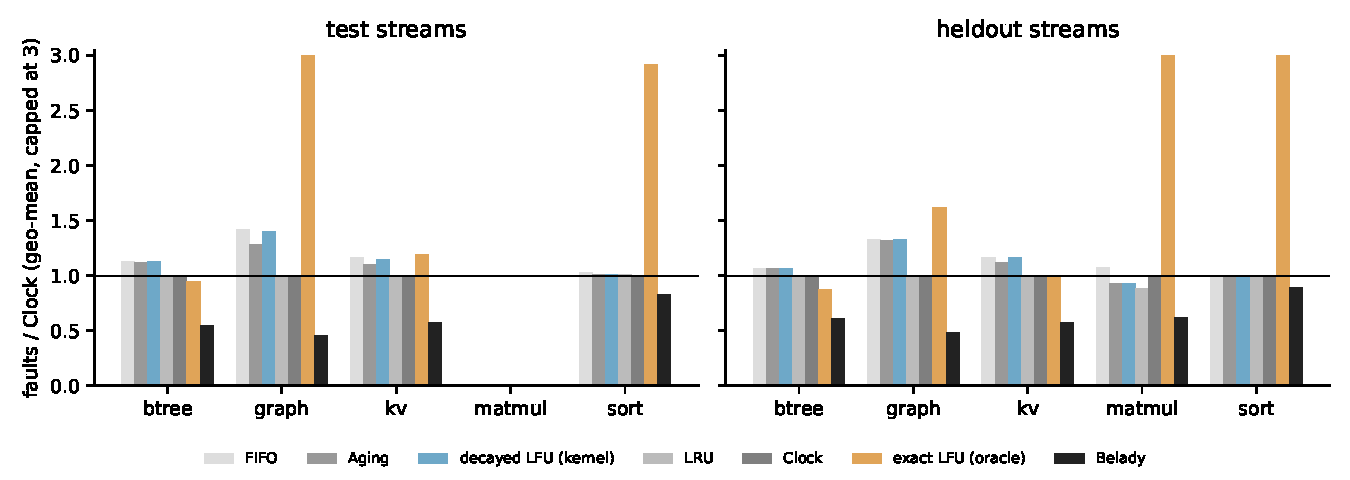
\includegraphics[width=\linewidth,height=.42\textheight,keepaspectratio]{figures2/classical.pdf}
\end{center}

\begin{itemize}
\item \textbf{Clock is within 1–2\% of LRU on four of the five workloads} (LRU is 0.98–1.01× Clock); on matmul's held-out variants LRU is 12\% better (0.88) and even Aging beats Clock (0.93). Clock is the reference throughout: it is xv6's best built-in policy on the other four workloads, and true LRU is not implementable in a kernel.
\item \textbf{xv6's Aging is barely better than FIFO} (btree 1.12 vs 1.13, graph 1.29 vs 1.42 on test). Its 8-bit history shifts once per eviction, so at the eviction rates these capacities produce it forgets everything within 8 evictions and falls back on load order.
\item \textbf{The kernel's decayed LFU (\code{GawwyDev} \code{d1d247f}) is no better than FIFO} (btree 1.13, graph 1.40, kv 1.15 on test, against FIFO's 1.13, 1.42, 1.16): the decay that fixed its livelock also takes away what made it LFU.
\item \textbf{Exact LFU is the only classical policy that beats Clock anywhere} (btree 0.94 test, 0.87 held-out) and is catastrophic elsewhere (graph, sort, matmul ≥ 3× Clock). Frequency is a real signal, but on its own it cannot let a page's history expire.
\item \textbf{The headroom is large}: Belady needs 43–54\% fewer faults than Clock on the database-, key-value-and graph-shaped workloads (btree 0.55, kv 0.57, graph 0.46 on test), 38\% on matmul (held-out), and only 10–17\% on sort.
\end{itemize}

\subsection*{6.2 Which features carry signal — at the moment of the decision}
\addcontentsline{toc}{subsection}{6.2 Which features carry signal — at the moment of the decision}

Each feature's rank correlation with the true next-use distance, computed \textbf{within each recorded eviction} and averaged over decisions (\code{report/\allowbreak{}results2/\allowbreak{}feature\_\allowbreak{}diagnostics.\allowbreak{}csv}):

\begin{center}
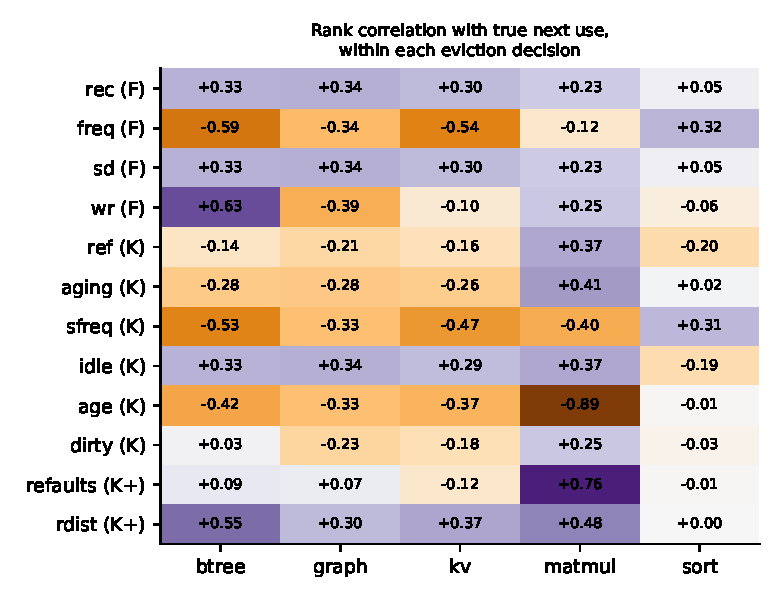
\includegraphics[width=\linewidth,height=.42\textheight,keepaspectratio]{figures2/diagnostics.pdf}
\end{center}

\begin{itemize}
\item \textbf{Kernel-observable signals nearly match the oracle ones.} The sampled access count \code{sfreq} (−0.45 btree, −0.44 kv) is almost as informative as the exact count \code{freq} (−0.52, −0.52), and the refault distance \code{rdist} — what Linux's workingset already measures — is as strong again (+0.45 btree, +0.36 graph, +0.35 kv).
\item \textbf{Recency and true stack distance are identical within a decision} (same values in every column), as §4 predicts.
\item \textbf{Pooled correlation misleads.} Recency's pooled Pearson correlation on sort is +0.87 but its within-decision rank correlation is +0.05 — sort's label is dominated by \emph{when} in the run a decision happens, which is the same for every candidate of that decision and so useless for choosing between them.
\end{itemize}

\subsection*{6.3 Every combination of the full-stream features}
\addcontentsline{toc}{subsection}{6.3 Every combination of the full-stream features}

All 15 subsets of \{\code{rec}, \code{freq}, \code{sd}, \code{wr}\}, linear, per-workload models, at 10\% (\code{report/\allowbreak{}results2/\allowbreak{}summary\_\allowbreak{}linear.\allowbreak{}csv}):

\tablecaption{\textbf{All 15 full-stream (F) subsets, linear, per-workload models, test, 10\% — faults / Clock}}

\begin{center}\footnotesize
\begin{adjustbox}{max width=\linewidth}
\begin{tabular}{lrrrrr}
\toprule
\textbf{features} & \textbf{btree} & \textbf{graph} & \textbf{kv} & \textbf{matmul} & \textbf{sort} \\ \midrule
rec & 0.999 & 0.976 & 0.986 & — & 0.954 \\
freq & 0.915 & ≥3.000 & 1.076 & — & 1.204 \\
sd & 0.999 & 0.976 & 0.986 & — & 0.954 \\
wr & 0.854 & ≥2.823 & ≥1.786 & — & 1.245 \\
rec+freq & 0.864 & 0.625 & 0.914 & — & 0.954 \\
rec+sd & 0.999 & 0.976 & 0.987 & — & 0.954 \\
rec+wr & 0.882 & 0.626 & 0.987 & — & 0.954 \\
freq+sd & 0.869 & ≥1.720 & 0.921 & — & 0.954 \\
freq+wr & 0.865 & ≥2.491 & 1.076 & — & 1.211 \\
sd+wr & 0.878 & ≥1.449 & 0.991 & — & 0.954 \\
rec+freq+sd & 0.888 & 0.636 & 0.912 & — & 0.954 \\
rec+freq+wr & 0.833 & 0.628 & 0.914 & — & 0.954 \\
rec+sd+wr & 0.873 & 0.656 & 0.991 & — & 0.954 \\
freq+sd+wr & 0.835 & ≥1.254 & 0.922 & — & 0.954 \\
rec+freq+sd+wr & 0.847 & 0.652 & 0.911 & — & 0.954 \\
\bottomrule
\end{tabular}
\end{adjustbox}
\end{center}

\tablecaption{\textbf{All 15 full-stream (F) subsets, linear, per-workload models, heldout, 10\% — faults / Clock}}

\begin{center}\footnotesize
\begin{adjustbox}{max width=\linewidth}
\begin{tabular}{lrrrrr}
\toprule
\textbf{features} & \textbf{btree} & \textbf{graph} & \textbf{kv} & \textbf{matmul} & \textbf{sort} \\ \midrule
rec & 0.995 & 0.999 & 0.983 & 0.999 & 1.000 \\
freq & 0.857 & 0.724 & 1.012 & 1.564 & 1.288 \\
sd & 0.995 & 0.999 & 0.983 & 0.999 & 1.000 \\
wr & 0.937 & 2.466 & 1.088 & 1.408 & 1.224 \\
rec+freq & 0.863 & 0.528 & 0.907 & 0.999 & 1.000 \\
rec+sd & 0.995 & 0.999 & 0.982 & 0.999 & 1.000 \\
rec+wr & 0.929 & 0.619 & 0.979 & 0.999 & 1.000 \\
freq+sd & 0.864 & 0.503 & 0.913 & 0.999 & 1.000 \\
freq+wr & 0.833 & 1.750 & 1.012 & 1.569 & 1.303 \\
sd+wr & 0.930 & 0.799 & 0.979 & 0.999 & 1.000 \\
rec+freq+sd & 0.865 & 0.519 & 0.906 & 0.999 & 1.000 \\
rec+freq+wr & 0.848 & 0.499 & 0.907 & 0.999 & 1.000 \\
rec+sd+wr & 0.930 & 0.620 & 0.979 & 0.999 & 1.000 \\
freq+sd+wr & 0.849 & 0.479 & 0.913 & 0.999 & 1.000 \\
rec+freq+sd+wr & 0.848 & 0.489 & 0.906 & 0.999 & 1.000 \\
\bottomrule
\end{tabular}
\end{adjustbox}
\end{center}

\begin{center}
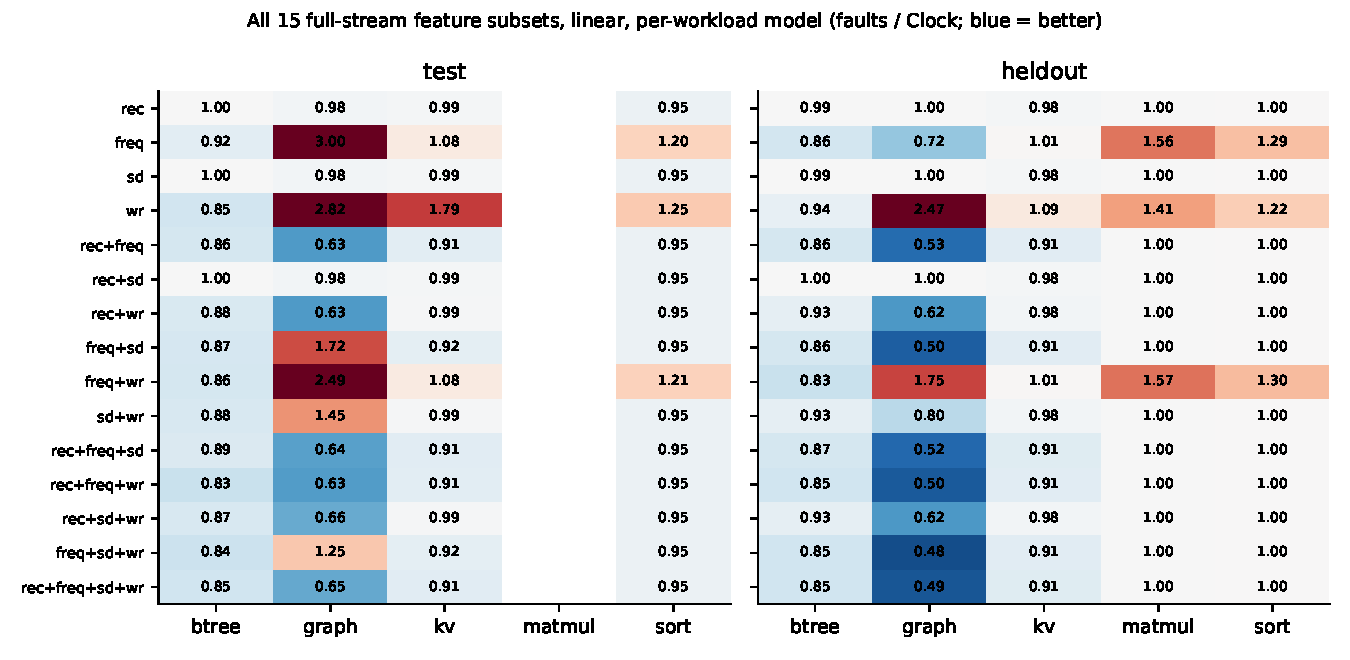
\includegraphics[width=\linewidth,height=.42\textheight,keepaspectratio]{figures2/f_subsets_workload.pdf}
\end{center}

\begin{itemize}
\item \textbf{A single feature is never enough.} Recency (or stack distance) alone reproduces LRU; frequency alone is catastrophic on graph (≥3×) and costs 20–56\% on sort and matmul; the write ratio alone is catastrophic on graph and 1.8× Clock on kv.
\item \textbf{Recency + frequency is the combination that matters} — graph 0.63 (test) and 0.53 (held-out), btree 0.86, kv 0.91. Adding the write ratio helps btree (0.83 with \code{rec+freq+wr}) and held-out graph (0.49–0.50); stack distance adds nothing once recency is present (they order pages alike).
\item \textbf{The global model is weaker than the per-workload one} on graph (0.68 vs 0.65 for all four; 0.76 vs 0.63 for \code{rec+freq}), and about equal elsewhere — one weight vector has to serve five behaviours.
\end{itemize}

\subsection*{6.4 Every combination of the kernel-observable features}
\addcontentsline{toc}{subsection}{6.4 Every combination of the kernel-observable features}

All 255 subsets of the eight K ∪ K+ features, per-workload models, 10\%:

\tablecaption{\textbf{The 255 kernel-observable (K ∪ K+) subsets, per-workload models, test, 10\% — distribution of faults / Clock}}

\begin{center}\footnotesize
\begin{adjustbox}{max width=\linewidth}
\begin{tabular}{lrrrrrr}
\toprule
\textbf{workload} & \textbf{best} & \textbf{10th pct} & \textbf{median} & \textbf{90th pct} & \textbf{beat Clock} & \textbf{≥3× Clock} \\ \midrule
btree & 0.797 & 0.820 & 0.932 & 1.772 & 152/255 & 0 \\
graph & 0.628 & 0.681 & 1.004 & 3.000 & 126/255 & 98 \\
kv & 0.888 & 0.907 & 1.012 & 1.759 & 122/255 & 0 \\
sort & 0.945 & 0.967 & 1.046 & 1.157 & 71/255 & 0 \\
\bottomrule
\end{tabular}
\end{adjustbox}
\end{center}

\tablecaption{\textbf{The 255 kernel-observable (K ∪ K+) subsets, per-workload models, heldout, 10\% — distribution of faults / Clock}}

\begin{center}\footnotesize
\begin{adjustbox}{max width=\linewidth}
\begin{tabular}{lrrrrrr}
\toprule
\textbf{workload} & \textbf{best} & \textbf{10th pct} & \textbf{median} & \textbf{90th pct} & \textbf{beat Clock} & \textbf{≥3× Clock} \\ \midrule
btree & 0.838 & 0.847 & 0.888 & 1.371 & 180/255 & 0 \\
graph & 0.485 & 0.497 & 0.684 & 1.837 & 176/255 & 8 \\
kv & 0.900 & 0.926 & 0.990 & 1.443 & 132/255 & 0 \\
matmul & 0.969 & 0.975 & 1.067 & 1.496 & 94/255 & 0 \\
sort & 0.950 & 0.998 & 1.007 & 1.174 & 28/255 & 0 \\
\bottomrule
\end{tabular}
\end{adjustbox}
\end{center}

\begin{center}
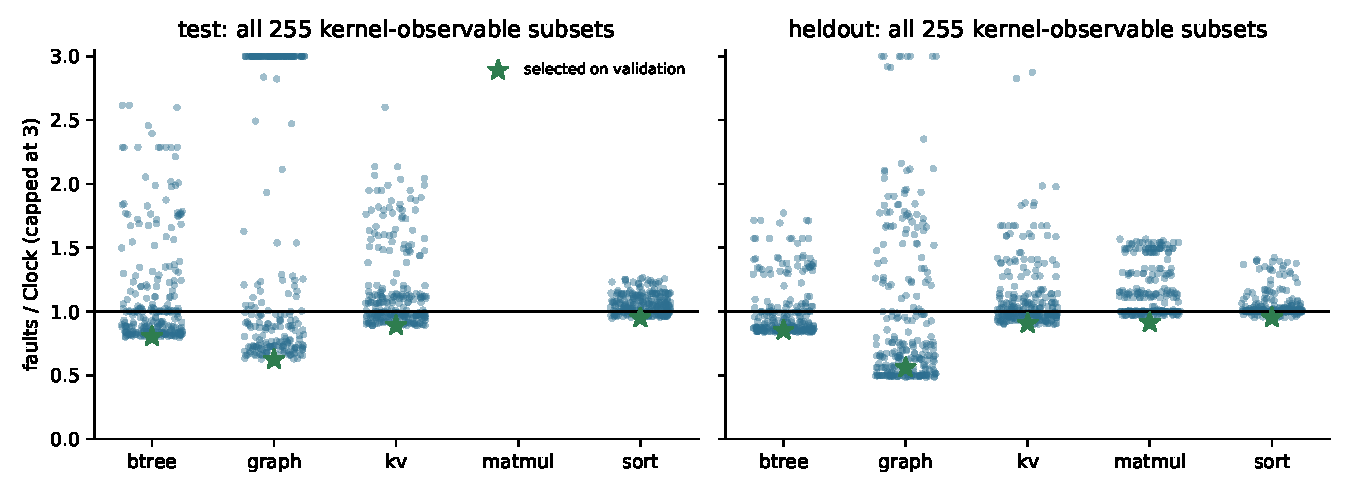
\includegraphics[width=\linewidth,height=.42\textheight,keepaspectratio]{figures2/kk_subsets.pdf}
\end{center}

What each kernel feature is worth — the median change in faults when it is added to a subset that lacks it, over all such pairs:

\tablecaption{\textbf{Median change in faults from adding one kernel feature to a subset that lacks it (per-workload models, test; matmul: held-out; over all such subset pairs)}}

\begin{center}\footnotesize
\begin{adjustbox}{max width=\linewidth}
\begin{tabular}{lrrrrr}
\toprule
\textbf{feature} & \textbf{btree} & \textbf{graph} & \textbf{kv} & \textbf{matmul} & \textbf{sort} \\ \midrule
ref & -0.1\% & +0.0\% & -0.2\% & +0.0\% & -0.9\% \\
aging & -1.6\% & +0.0\% & -1.7\% & -0.5\% & -2.5\% \\
sfreq & -8.9\% & +2.7\% & +3.4\% & +2.4\% & +6.9\% \\
idle & -29.2\% & -70.8\% & -19.5\% & -21.8\% & +0.0\% \\
age & -1.1\% & +0.0\% & -2.0\% & +0.4\% & +1.6\% \\
dirty & -2.2\% & -3.4\% & +0.4\% & +0.0\% & -0.1\% \\
refaults & -5.4\% & +0.0\% & -2.6\% & +0.0\% & -5.0\% \\
rdist & +0.6\% & +0.0\% & +1.0\% & +0.0\% & +0.4\% \\
\bottomrule
\end{tabular}
\end{adjustbox}
\end{center}

\begin{center}
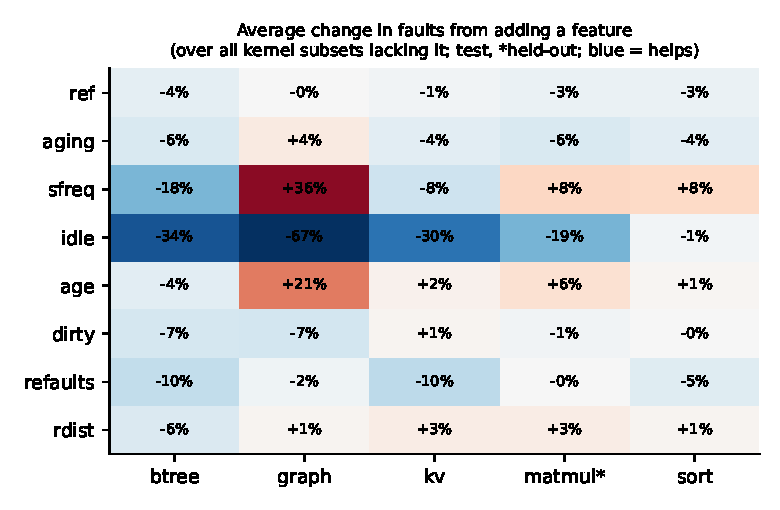
\includegraphics[width=\linewidth,height=.42\textheight,keepaspectratio]{figures2/marginal.pdf}
\end{center}

\begin{itemize}
\item \textbf{The best kernel-observable subsets match or beat the best oracle subsets}: btree 0.80 vs 0.83, graph 0.63 vs 0.63 (held-out 0.49 vs 0.48), kv 0.89 vs 0.91, sort 0.95 vs 0.95 (best-of-set on test; the honest, validation-selected numbers are in §6.5). \textbf{The information a kernel can collect from accessed/dirty-bit scans is enough} to express what the oracle features express here.
\item \textbf{\code{idle} — scans since the page was last found accessed — is by far the most valuable kernel feature}: adding it cuts faults by a median 71\% on graph, 29\% on btree, 20\% on kv, 22\% on matmul. It is the kernel's own recency signal, and it is what Linux's MGLRU generations and DAMON's age already track.
\item \textbf{Selection matters as much as the model.} More than half of the 255 subsets are worse than Clock on kv and sort, and on graph 98 (per-workload) to 126 (global) are catastrophic at 10\%. A learned policy is only as good as the feature set and the validation that chose it.
\end{itemize}

\subsection*{6.5 Headline: validation-selected models, every tier}
\addcontentsline{toc}{subsection}{6.5 Headline: validation-selected models, every tier}

The best model of each tier, chosen by nested selection on validation (§5.5), then replayed once on test (unseen seeds) and held-out (unseen variants) at 5\%, 10\% and 20\% — geometric mean over the three capacities; in brackets, the share of the Clock→Belady gap closed:

\tablecaption{\textbf{Validation-selected linear model per tier (per-workload model), test — faults / Clock, geo-mean over 5/10/20\% (share of the Clock→Belady gap closed)}}

\begin{center}\footnotesize
\begin{adjustbox}{max width=\linewidth}
\begin{tabular}{lrrrrrr}
\toprule
\textbf{workload} & \textbf{LRU} & \textbf{oracle (F)} & \textbf{kernel (K)} & \textbf{kernel+refault (K∪K+)} & \textbf{oracle+kernel} & \textbf{Belady} \\ \midrule
btree & 0.994 & 0.861 (+32\%) & 0.852 (+33\%) & 0.833 (+38\%) & 0.845 (+35\%) & 0.550 \\
graph & 0.990 & 0.855 (+22\%) & 0.871 (+21\%) & 0.845 (+26\%) & 0.855 (+22\%) & 0.456 \\
kv & 0.986 & 0.910 (+21\%) & 0.917 (+19\%) & 0.905 (+22\%) & 0.937 (+15\%) & 0.571 \\
sort & 1.012 & 1.011 (+12\%) & 1.011 (+11\%) & 0.983 (+30\%) & 0.947 (+30\%) & 0.830 \\
\bottomrule
\end{tabular}
\end{adjustbox}
\end{center}

\tablenote{\emph{Feature subset and probation chosen on validation only (matmul: its training streams).}}

\tablecaption{\textbf{Validation-selected linear model per tier (per-workload model), heldout — faults / Clock, geo-mean over 5/10/20\% (share of the Clock→Belady gap closed)}}

\begin{center}\footnotesize
\begin{adjustbox}{max width=\linewidth}
\begin{tabular}{lrrrrrr}
\toprule
\textbf{workload} & \textbf{LRU} & \textbf{oracle (F)} & \textbf{kernel (K)} & \textbf{kernel+refault (K∪K+)} & \textbf{oracle+kernel} & \textbf{Belady} \\ \midrule
btree & 0.997 & 0.861 (+38\%) & 0.893 (+29\%) & 0.863 (+37\%) & 0.864 (+37\%) & 0.615 \\
graph & 0.992 & 0.786 (+31\%) & 0.805 (+29\%) & 0.798 (+30\%) & 0.767 (+34\%) & 0.482 \\
kv & 0.982 & 0.890 (+27\%) & 0.916 (+21\%) & 0.905 (+23\%) & 0.922 (+19\%) & 0.577 \\
matmul & 0.879 & 0.823 (+26\%) & 0.789 (+39\%) & 0.681 (+73\%) & 0.751 (+44\%) & 0.617 \\
sort & 0.999 & 0.999 (+4\%) & 0.999 (+4\%) & 0.933 (+51\%) & 1.001 (+0\%) & 0.896 \\
\bottomrule
\end{tabular}
\end{adjustbox}
\end{center}

\tablenote{\emph{Feature subset and probation chosen on validation only (matmul: its training streams).}}

\begin{center}
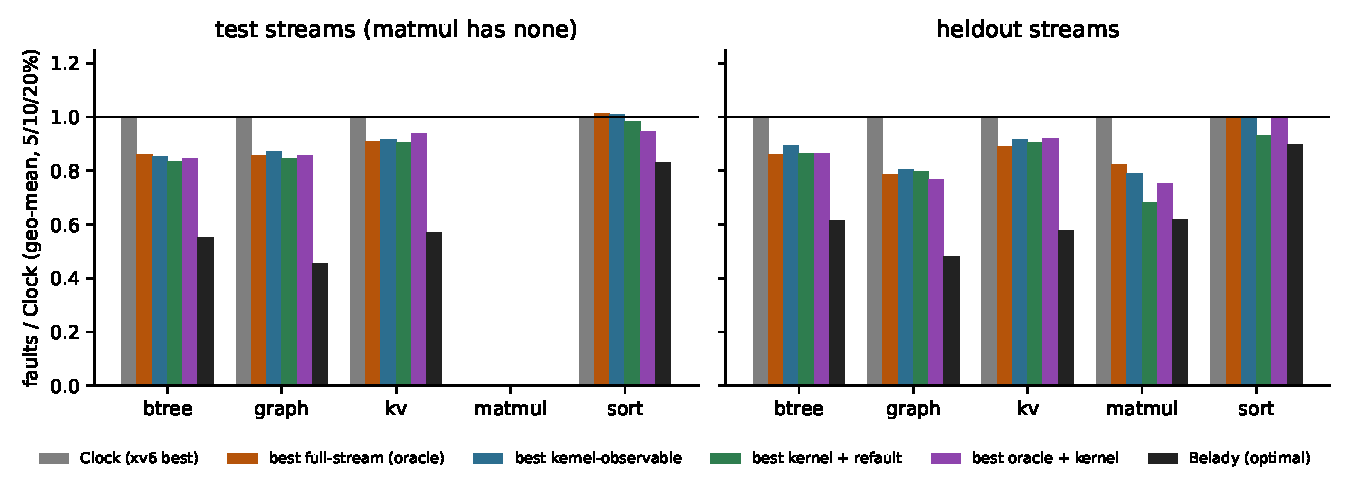
\includegraphics[width=\linewidth,height=.42\textheight,keepaspectratio]{figures2/tiers_workload.pdf}
\end{center}

The models chosen (feature subset, probation in scans):

\tablecaption{\textbf{Models chosen on validation: feature subset (probation, in scans)}}

\begin{center}\footnotesize
\begin{tabularx}{\linewidth}{llXXX}
\toprule
\textbf{scope} & \textbf{oracle (F)} & \textbf{kernel (K)} & \textbf{kernel+refault (K∪K+)} & \textbf{oracle+kernel} \\ \midrule
btree & rec + freq + wr (0) & ref + idle + age + dirty (0) & aging + idle + age + dirty + refaults (0) & rec + ref + aging + sfreq + idle + age + dirty (1) \\
graph & rec + freq (4) & sfreq + idle + dirty (4) & sfreq + idle + dirty + rdist (4) & rec + ref + aging + sfreq + idle + age + dirty (4) \\
kv & rec + freq + sd + wr (2) & ref + aging + idle + age (4) & aging + idle + dirty + refaults + rdist (2) & freq + wr + ref + aging + sfreq + idle + age + dirty (2) \\
matmul & rec + wr (0) & ref + aging + idle + dirty (0) & aging + idle + dirty + refaults + rdist (0) & sd + ref + aging + sfreq + idle + age + dirty (0) \\
sort & rec + freq + sd (2) & aging (0) & ref + dirty + refaults + rdist (4) & rec + sd + ref + aging + sfreq + idle + age + dirty + refaults + rdist (2) \\
global & rec + freq + sd + wr (0) & aging + idle + age (0) & idle + dirty + refaults + rdist (4) & rec + ref + aging + sfreq + idle + age + dirty (0) \\
\bottomrule
\end{tabularx}
\end{center}

\begin{itemize}
\item \textbf{Kernel-observable features are enough.} With only what a kernel can collect — accessed/dirty-bit scan history plus refault bookkeeping — the selected policy beats Clock on \textbf{every workload, on unseen seeds and on unseen variants}: btree −17\% faults (test) / −14\% (held-out), graph −15\% / −20\%, kv −10\% / −10\%, matmul −32\% (held-out), sort −2\% / −7\%. That closes 22–38\% of the gap to Belady on test and 23–73\% on held-out.
\item \textbf{The oracle features buy almost nothing over them.} On btree, graph and kv the best full-stream model is within ±1.5\% of the kernel+refault model — slightly behind on test (btree 0.861 vs 0.833, graph 0.855 vs 0.845, kv 0.910 vs 0.905), slightly ahead on held-out (0.861 vs 0.863, 0.786 vs 0.798, 0.890 vs 0.905) — and it is far behind on matmul (0.823 vs 0.681) and sort held-out (0.999 vs 0.933). Joining oracle and kernel features does not help either. For these workloads, what the kernel cannot see is not what limits a learned policy.
\item \textbf{Refault bookkeeping is worth adding.} K∪K+ beats K-only in all 9 workload × split cells (e.g. matmul 0.681 vs 0.789, sort held-out 0.933 vs 0.999).
\item \textbf{\code{idle} is in every kernel selection except sort's}, and probation is chosen long on graph (4 scans), short on kv (2–4) and off on btree and matmul (0).
\item \textbf{Generalisation holds.} Held-out variants — behaviours never seen in training — are not worse than test seeds: the gap closed is higher on graph, kv and sort, and within one point on btree.
\end{itemize}

\textbf{One model for every program.} A kernel does not know which program is running, so the realistic deployment is the global model:

\tablecaption{\textbf{Validation-selected linear model per tier (one global model), test — faults / Clock, geo-mean over 5/10/20\% (share of the Clock→Belady gap closed)}}

\begin{center}\footnotesize
\begin{adjustbox}{max width=\linewidth}
\begin{tabular}{lrrrrrr}
\toprule
\textbf{workload} & \textbf{LRU} & \textbf{oracle (F)} & \textbf{kernel (K)} & \textbf{kernel+refault (K∪K+)} & \textbf{oracle+kernel} & \textbf{Belady} \\ \midrule
btree & 0.994 & 0.900 (+23\%) & 0.887 (+25\%) & 0.864 (+31\%) & 0.891 (+24\%) & 0.550 \\
graph & 0.990 & 0.873 (+20\%) & 0.851 (+22\%) & 0.874 (+11\%) & 0.892 (+18\%) & 0.456 \\
kv & 0.986 & 0.920 (+19\%) & 0.920 (+18\%) & 0.908 (+22\%) & 0.944 (+13\%) & 0.571 \\
sort & 1.012 & 0.967 (+25\%) & 1.019 (+6\%) & 1.005 (+13\%) & 0.933 (+34\%) & 0.830 \\
\bottomrule
\end{tabular}
\end{adjustbox}
\end{center}

\tablenote{\emph{Feature subset and probation chosen on validation only (matmul: its training streams).}}

\tablecaption{\textbf{Validation-selected linear model per tier (one global model), heldout — faults / Clock, geo-mean over 5/10/20\% (share of the Clock→Belady gap closed)}}

\begin{center}\footnotesize
\begin{adjustbox}{max width=\linewidth}
\begin{tabular}{lrrrrrr}
\toprule
\textbf{workload} & \textbf{LRU} & \textbf{oracle (F)} & \textbf{kernel (K)} & \textbf{kernel+refault (K∪K+)} & \textbf{oracle+kernel} & \textbf{Belady} \\ \midrule
btree & 0.997 & 0.922 (+21\%) & 0.924 (+20\%) & 0.898 (+28\%) & 0.927 (+19\%) & 0.615 \\
graph & 0.992 & 0.855 (+23\%) & 0.815 (+27\%) & 0.792 (+29\%) & 0.948 (+6\%) & 0.482 \\
kv & 0.982 & 0.903 (+24\%) & 0.919 (+20\%) & 0.901 (+24\%) & 0.933 (+16\%) & 0.577 \\
matmul & 0.879 & 0.872 (+18\%) & 0.814 (+27\%) & 0.967 (-60\%) & 0.817 (+27\%) & 0.617 \\
sort & 0.999 & 0.998 (+5\%) & 0.999 (+4\%) & 0.966 (+24\%) & 0.999 (+4\%) & 0.896 \\
\bottomrule
\end{tabular}
\end{adjustbox}
\end{center}

\tablenote{\emph{Feature subset and probation chosen on validation only (matmul: its training streams).}}

\begin{center}
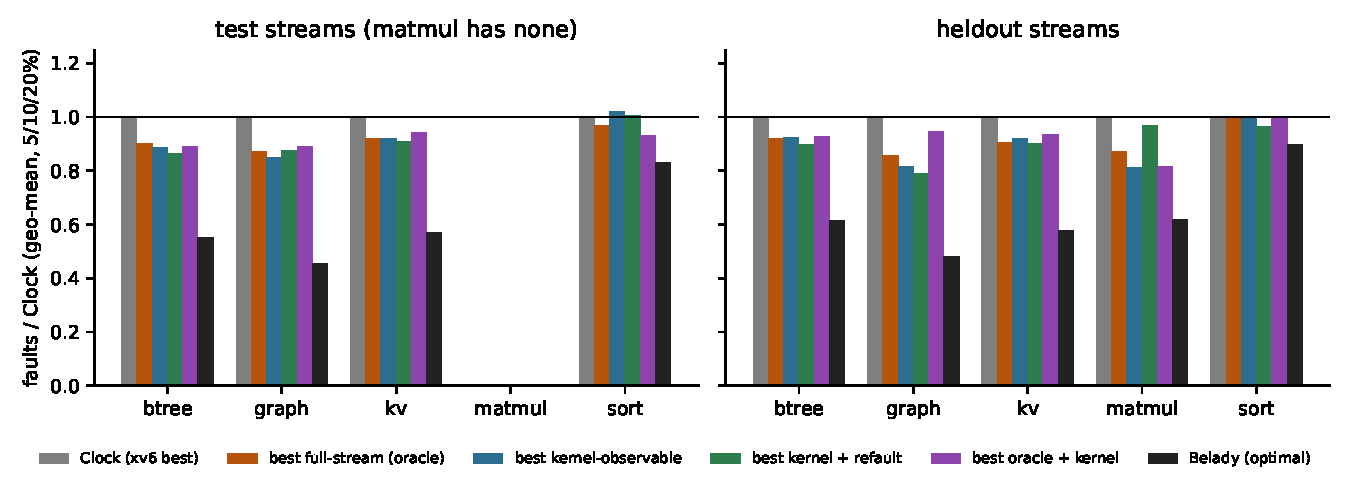
\includegraphics[width=\linewidth,height=.42\textheight,keepaspectratio]{figures2/tiers_global.pdf}
\end{center}

The single global kernel+refault model still beats Clock on 8 of 9 workload × split cells (btree 0.864 / 0.898, graph 0.874 / 0.792, kv 0.908 / 0.901, matmul 0.967, sort 1.005 / 0.966). It keeps most of the per-workload gain on btree, graph and kv but little of it on matmul (0.967 vs 0.681). The kernel-only global model is better than it on two cells (graph test 0.851, matmul 0.814). A per-program or per-phase choice of weights is the obvious next step (§10).

\textbf{By capacity.} The gains depend on memory pressure, most of all on graph:

\tablecaption{\textbf{By capacity: the selected kernel+refault (K∪K+) model (per-workload) — faults / Clock}}

\begin{center}\footnotesize
\begin{adjustbox}{max width=\linewidth}
\begin{tabular}{llrrrrrr}
\toprule
\textbf{workload} & \textbf{split} & \textbf{5\%} & \textbf{10\%} & \textbf{20\%} & \textbf{Belady 5\%} & \textbf{Belady 10\%} & \textbf{Belady 20\%} \\ \midrule
btree & test & 0.804 & 0.803 & 0.895 & 0.608 & 0.550 & 0.498 \\
btree & heldout & 0.853 & 0.854 & 0.882 & 0.686 & 0.627 & 0.541 \\
graph & test & 0.979 & 0.624 & 0.986 & 0.412 & 0.337 & 0.682 \\
graph & heldout & 0.931 & 0.560 & 0.976 & 0.477 & 0.377 & 0.623 \\
kv & test & 0.867 & 0.890 & 0.960 & 0.629 & 0.573 & 0.516 \\
kv & heldout & 0.841 & 0.907 & 0.970 & 0.617 & 0.588 & 0.530 \\
matmul & heldout & 0.500 & 0.913 & 0.692 & 0.500 & 0.839 & 0.560 \\
sort & test & 1.099 & 0.950 & 0.912 & 0.758 & 0.897 & 0.842 \\
sort & heldout & 0.994 & 0.951 & 0.859 & 0.959 & 0.918 & 0.818 \\
\bottomrule
\end{tabular}
\end{adjustbox}
\end{center}

On graph the selected model's gain is concentrated at 10\% (0.62 test, 0.56 held-out); at 5\% and 20\% it is within 2–7\% of Clock even though Belady still has large headroom there (0.41 at 5\%). This is not a selection artefact: probing graph's validation streams at 5\% and 20\% with every promising subset, each probation setting, and models trained only on data from that capacity, no linear model gets below 0.93. At those capacities what Belady exploits is not expressible as a linear score of these per-page features. On btree, kv and sort the gains are spread across capacities; on matmul they are largest at 5\% (0.50 — matching Belady).

\subsection*{6.6 Disk writes}
\addcontentsline{toc}{subsection}{6.6 Disk writes}

Fewer faults is half the story for a paging system: an eviction that has to write the page back costs a disk write. Page writes relative to Clock:

\tablecaption{\textbf{Page writes (disk writebacks) relative to Clock, geo-mean over 5/10/20\%}}

\begin{center}\footnotesize
\begin{adjustbox}{max width=\linewidth}
\begin{tabular}{llrrrr}
\toprule
\textbf{workload} & \textbf{split} & \textbf{LRU} & \textbf{kernel+refault} & \textbf{oracle} & \textbf{Belady} \\ \midrule
btree & test & 0.997 & 0.967 & 0.932 & 0.707 \\
btree & heldout & 0.997 & 0.965 & 0.962 & 0.646 \\
graph & test & 0.938 & 0.418 & 0.578 & 0.257 \\
graph & heldout & 0.727 & 0.338 & 0.616 & 0.297 \\
kv & test & 0.975 & 0.819 & 0.856 & 0.690 \\
kv & heldout & 0.982 & 0.904 & 0.890 & 0.574 \\
matmul & heldout & 1.008 & 0.658 & 1.008 & 0.863 \\
sort & test & 1.016 & 0.987 & 1.015 & 0.868 \\
sort & heldout & 1.000 & 0.935 & 1.000 & 0.932 \\
\bottomrule
\end{tabular}
\end{adjustbox}
\end{center}

\tablenote{\emph{Below 1: fewer writes than Clock. Belady minimises faults, not writes.}}

The learned kernel policy reduces \textbf{writes much more than faults} — graph 0.42 / 0.34 of Clock's page writes, matmul 0.66, kv 0.82 / 0.90 — because the selected subsets use the dirty bit and keep written pages resident. On graph it cuts writes by 58–66\% while Belady, which minimises faults and ignores writes, cuts them by 70–74\%.

\subsection*{6.7 Neural, sequence and ranking models}
\addcontentsline{toc}{subsection}{6.7 Neural, sequence and ranking models}

At 10\%, every neural model with its probation (0 or 2 scans) chosen on validation, next to the validation-selected linear kernel+refault model:

\tablecaption{\textbf{Neural and ranking-loss scorers (per-workload models), test, 10\% — faults / Clock}}

\begin{center}\footnotesize
\begin{adjustbox}{max width=\linewidth}
\begin{tabular}{lrrrrrrrrr}
\toprule
\textbf{workload} & \textbf{linear K∪K+ (sel.)} & \textbf{MLP F} & \textbf{rank-MLP F} & \textbf{MLP K∪K+} & \textbf{rank-MLP K∪K+} & \textbf{rank-linear K∪K+} & \textbf{MLP all} & \textbf{GRU (F)} & \textbf{embedding (F)} \\ \midrule
btree & 0.803 & 0.798 & 0.800 & 0.786 & 1.014 & 1.006 & 0.792 & 0.784 & ≥2.456 \\
graph & 0.624 & 0.627 & 0.643 & 0.622 & ≥1.699 & 0.669 & 0.641 & 0.632 & ≥3.000 \\
kv & 0.890 & 0.899 & 0.976 & 0.852 & 0.887 & 0.943 & 0.835 & 0.854 & 0.847 \\
sort & 0.950 & 0.955 & 1.016 & 0.965 & 1.192 & 1.234 & 0.939 & 0.957 & 1.103 \\
\bottomrule
\end{tabular}
\end{adjustbox}
\end{center}

\tablenote{\emph{Probation (0 or 2 scans) chosen per model on validation.}}

\tablecaption{\textbf{Neural and ranking-loss scorers (per-workload models), heldout, 10\% — faults / Clock}}

\begin{center}\footnotesize
\begin{adjustbox}{max width=\linewidth}
\begin{tabular}{lrrrrrrrrr}
\toprule
\textbf{workload} & \textbf{linear K∪K+ (sel.)} & \textbf{MLP F} & \textbf{rank-MLP F} & \textbf{MLP K∪K+} & \textbf{rank-MLP K∪K+} & \textbf{rank-linear K∪K+} & \textbf{MLP all} & \textbf{GRU (F)} & \textbf{embedding (F)} \\ \midrule
btree & 0.854 & 0.864 & 0.833 & 0.884 & 0.932 & 0.928 & 0.832 & 0.831 & 1.483 \\
graph & 0.560 & 0.473 & 0.625 & 0.495 & 1.109 & 0.491 & 0.480 & 0.484 & ≥3.000 \\
kv & 0.907 & 0.906 & 0.960 & 0.850 & 0.858 & 0.934 & 0.868 & 0.982 & 0.817 \\
matmul & 0.913 & 0.999 & ≥1.680 & 0.966 & 0.923 & 1.496 & 0.964 & 0.969 & ≥1.792 \\
sort & 0.951 & 1.001 & 1.044 & 0.998 & 1.244 & 1.268 & 0.977 & 1.000 & 1.171 \\
\bottomrule
\end{tabular}
\end{adjustbox}
\end{center}

\tablenote{\emph{Probation (0 or 2 scans) chosen per model on validation.}}

\begin{center}
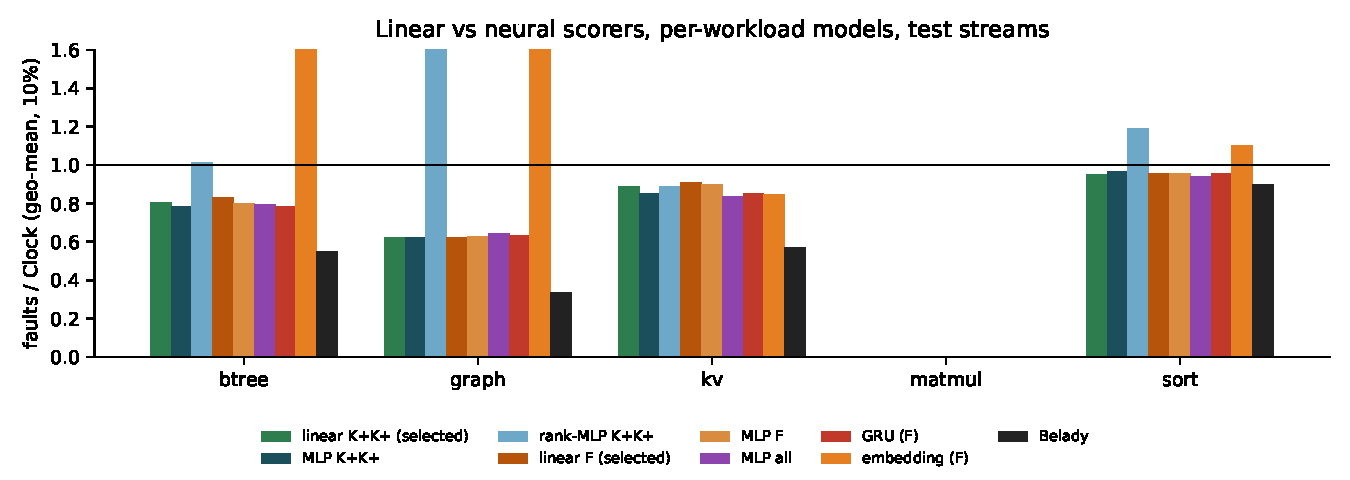
\includegraphics[width=\linewidth,height=.42\textheight,keepaspectratio]{figures2/nn_test.pdf}
\end{center}

\begin{center}
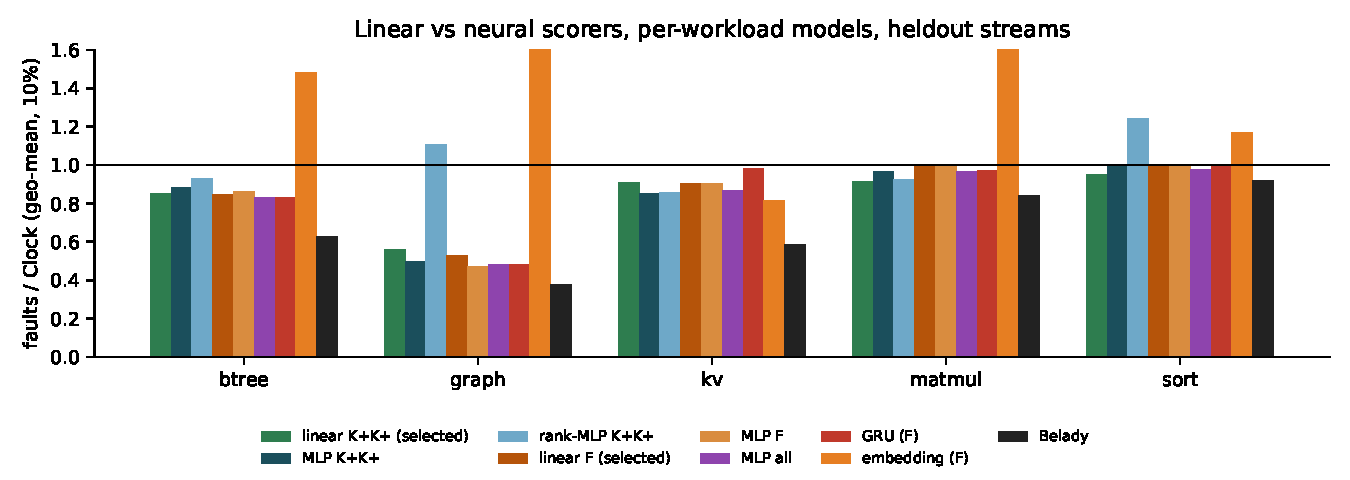
\includegraphics[width=\linewidth,height=.42\textheight,keepaspectratio]{figures2/nn_heldout.pdf}
\end{center}

\begin{itemize}
\item \textbf{A linear score is competitive with everything tried.} An MLP over the same kernel+refault features is better on kv (0.852 vs 0.890 test, 0.850 vs 0.907 held-out) and held-out graph (0.495 vs 0.560), about equal on test graph and btree, and worse on held-out btree (0.884 vs 0.854) and matmul (0.966 vs 0.913). There is some nonlinear signal in kv's hot-set rotation, but not enough to justify \textasciitilde{}260× the arithmetic per candidate in a kernel (≈1,300 multiply-adds for 8→32→32→1 against 5).
\item \textbf{The oracle GRU over each page's access intervals is no better than the linear models} (btree 0.784, graph 0.632, kv 0.854 on test): a richer view of a page's own history adds little once recency, frequency and write ratio are available.
\item \textbf{The cross-page embedding model} (a learned vector per page plus the last 16 pages referenced by the whole program) \textbf{is catastrophic on btree and graph} — page identities do not transfer across seeds there — and the \emph{best} model of all on held-out kv (0.817). In the key-value store, which pages are hot is a property of the pages themselves; elsewhere it is not. It is an oracle ablation: a kernel has neither the global reference window nor floating point.
\item \textbf{The ranking loss did not help.} Training on a softmax over each decision's candidates towards Belady's choice is worse than regressing the log distance for most model × workload cells (e.g. rank-MLP K∪K+: btree 1.014, sort 1.192 on test). Regression on the full distance carries more information than ``which one is furthest''.
\end{itemize}

The global versions tell the same story with smaller margins:

\tablecaption{\textbf{Neural and ranking-loss scorers (global models), test, 10\% — faults / Clock}}

\begin{center}\footnotesize
\begin{adjustbox}{max width=\linewidth}
\begin{tabular}{lrrrrrrrrr}
\toprule
\textbf{workload} & \textbf{linear K∪K+ (sel.)} & \textbf{MLP F} & \textbf{rank-MLP F} & \textbf{MLP K∪K+} & \textbf{rank-MLP K∪K+} & \textbf{rank-linear K∪K+} & \textbf{MLP all} & \textbf{GRU (F)} & \textbf{embedding (F)} \\ \midrule
btree & 0.841 & 0.829 & 0.804 & 0.798 & 0.889 & 0.801 & 0.800 & 0.796 & 2.223 \\
graph & 0.660 & 0.615 & 0.777 & 0.635 & 0.896 & 1.049 & 0.786 & 0.596 & ≥3.000 \\
kv & 0.892 & 0.938 & 1.028 & 0.950 & 1.009 & 1.175 & 0.899 & 0.895 & 1.011 \\
sort & 0.967 & 0.945 & 0.999 & 1.048 & 1.127 & 1.221 & 0.919 & 0.956 & 0.973 \\
\bottomrule
\end{tabular}
\end{adjustbox}
\end{center}

\tablenote{\emph{Probation (0 or 2 scans) chosen per model on validation.}}

\tablecaption{\textbf{Neural and ranking-loss scorers (global models), heldout, 10\% — faults / Clock}}

\begin{center}\footnotesize
\begin{adjustbox}{max width=\linewidth}
\begin{tabular}{lrrrrrrrrr}
\toprule
\textbf{workload} & \textbf{linear K∪K+ (sel.)} & \textbf{MLP F} & \textbf{rank-MLP F} & \textbf{MLP K∪K+} & \textbf{rank-MLP K∪K+} & \textbf{rank-linear K∪K+} & \textbf{MLP all} & \textbf{GRU (F)} & \textbf{embedding (F)} \\ \midrule
btree & 0.894 & 0.867 & 0.866 & 0.867 & 0.885 & 0.856 & 0.830 & 0.846 & 1.218 \\
graph & 0.515 & 0.467 & 0.564 & 0.659 & 0.574 & 0.914 & 0.461 & 0.449 & 2.927 \\
kv & 0.900 & 1.046 & 1.157 & 0.992 & 1.004 & 0.994 & 0.907 & 1.133 & 0.955 \\
matmul & 1.338 & 0.999 & 1.355 & 0.906 & 1.201 & 1.430 & 0.936 & 0.969 & 1.628 \\
sort & 0.985 & 0.985 & 1.064 & 1.371 & 1.142 & 1.345 & 0.956 & 1.005 & ≥3.000 \\
\bottomrule
\end{tabular}
\end{adjustbox}
\end{center}

\tablenote{\emph{Probation (0 or 2 scans) chosen per model on validation.}}

\section*{7. What went wrong, and the fixes}
\addcontentsline{toc}{section}{7. What went wrong, and the fixes}

\subsection*{7.1 The first training set taught models to evict the page being streamed}
\addcontentsline{toc}{subsection}{7.1 The first training set taught models to evict the page being streamed}

The first version of the study (v1: \code{report/\allowbreak{}results2/\allowbreak{}linear\_\allowbreak{}sweep\_\allowbreak{}v1.\allowbreak{}csv}) recorded Belady's choice plus 31 \emph{uniformly random} candidates per sampled eviction. On \code{graph-pr2000x2} (PageRank alone) almost every linear model was catastrophic — ≥3× Clock — even one fitted on PageRank training decisions alone, and three DAgger rounds (≈2.4M rows recorded under the model's own decisions) did not help.

Looking at the decisions such a policy actually makes (\code{graph-pr2000x2-s2}, validation): \textbf{97\% of its victims were loaded at the immediately preceding fault, and their next use was a median of 16 references away} — the page the program was streaming through — while Belady's choice at the same decisions had last been used \textasciitilde{}300 references earlier. Each fault evicted the page that would be needed next, which faulted it straight back in.

The cause was the training data, not the model. Out of 167 resident pages, the one or two that were just touched are almost never among 31 uniform samples, so the models never saw a ``just used — keep it'' example and extrapolated badly there. DAgger could not fix it because it records with the same sampler. It is the same pathology as the kernel LFU livelock (a fresh page looks coldest), reached by a different route.

\subsection*{7.2 Two fixes, both chosen on validation}
\addcontentsline{toc}{subsection}{7.2 Two fixes, both chosen on validation}

\begin{enumerate}
\item \textbf{Recency-stratified recording}: of the 32 recorded candidates, always include the 4 most recently accessed (share of just-accessed rows 0.6\% → 3.1\%).
\item \textbf{Probation}: a page loaded fewer than \emph{p} scans ago is not evicted while an older candidate exists. This is Clock's second chance for a new page; in the kernel it is one comparison per candidate.
\end{enumerate}

On PageRank validation at 10\% the all-features model (v1 data) goes from ≥3.0 to 0.85 with \emph{p} = 2, with no change on the other graph variants, kv or btree. Probation has a cost at tiny capacities (matmul has 5 frames at 10\%: holding the 2 newest out of the choice removes much of it), so \emph{p} is chosen per scope on validation (§5.5), not fixed.

\tablecaption{\textbf{Probation ablation (per-workload linear models, validation streams, 10\%; matmul: its training streams) — faults / Clock}}

\begin{center}\footnotesize
\begin{adjustbox}{max width=\linewidth}
\begin{tabular}{llrrrr}
\toprule
\textbf{workload} & \textbf{features} & \textbf{0} & \textbf{1} & \textbf{2} & \textbf{4} \\ \midrule
btree & F & 0.853 & 0.853 & 0.853 & 0.853 \\
btree & K & 0.821 & 0.821 & 0.821 & 0.821 \\
btree & K∪K+ & 0.838 & 0.838 & 0.839 & 0.839 \\
btree & all & 1.007 & 1.011 & 1.005 & 1.008 \\
graph & F & 0.812 & 0.671 & 0.644 & 0.625 \\
graph & K & 0.794 & 0.732 & 0.706 & 0.673 \\
graph & K∪K+ & ≥1.105 & ≥1.101 & 1.029 & 1.008 \\
graph & all & 0.810 & 0.628 & 0.618 & 0.613 \\
kv & F & 0.914 & 0.913 & 0.912 & 0.912 \\
kv & K & 0.956 & 0.955 & 0.955 & 0.955 \\
kv & K∪K+ & 0.976 & 0.958 & 0.959 & 0.959 \\
kv & all & 0.993 & 0.982 & 0.978 & 0.980 \\
matmul & F & 0.738 & 0.861 & 0.938 & 0.845 \\
matmul & K & 0.639 & 0.835 & 0.975 & 0.704 \\
matmul & K∪K+ & 0.626 & 0.829 & 0.974 & 0.841 \\
matmul & all & ≥0.905 & 0.857 & 0.879 & 0.780 \\
sort & F & 0.960 & 0.960 & 0.960 & 0.965 \\
sort & K & 1.055 & 1.055 & 1.055 & 1.014 \\
sort & K∪K+ & 1.036 & 1.036 & 1.036 & 1.008 \\
sort & all & 0.964 & 0.964 & 0.962 & 0.969 \\
\bottomrule
\end{tabular}
\end{adjustbox}
\end{center}

Probation is decisive on graph — faults fall steadily with a longer probation (all features: 0.810 → 0.613 from 0 to 4 scans) — harmful on matmul (kernel+refault 0.626 → 0.974 at 2 scans; holding the newest pages out of a 5-frame choice leaves little choice), and irrelevant on btree, kv and sort (within 0.5\%). The selected models reflect this: 4 scans on graph, 2–4 on kv, 0 on btree and matmul.

Effect of the two fixes on the same fixed feature groups, compared on identical stream × capacity cells:

\tablecaption{\textbf{Effect of the two fixes on the same linear models (per-workload, 10\%) — faults / Clock; v1: uniform candidate sampling, no probation; v2: recency-stratified sampling + probation 2}}

{\footnotesize\setlength{\tabcolsep}{4pt}
\begin{longtable}{lllrr}
\toprule
\textbf{workload} & \textbf{split} & \textbf{features} & \textbf{v1} & \textbf{v2} \\ \midrule
\endhead
btree & heldout & F & 0.853 & 0.849 \\
btree & heldout & K & 0.849 & 0.851 \\
btree & heldout & K∪K+ & 0.847 & 0.846 \\
btree & heldout & all & 0.899 & 0.877 \\
graph & val & F & ≥1.258 & 0.707 \\
graph & val & K & ≥1.273 & 0.809 \\
graph & val & K∪K+ & ≥1.334 & 1.383 \\
graph & val & all & ≥1.257 & 0.661 \\
graph & test & F & ≥1.255 & 0.720 \\
graph & test & K & ≥1.268 & 0.806 \\
graph & test & K∪K+ & ≥1.330 & 1.463 \\
graph & test & all & ≥1.254 & 0.669 \\
kv & val & F & 0.964 & 0.960 \\
kv & val & K & 0.986 & 1.003 \\
kv & val & K∪K+ & 0.994 & 0.991 \\
kv & val & all & 1.020 & 1.042 \\
kv & test & F & 0.959 & 0.956 \\
kv & test & K & 0.987 & 1.004 \\
kv & test & K∪K+ & 0.997 & 0.986 \\
kv & test & all & 1.030 & 1.042 \\
matmul & heldout & F & 1.001 & 0.999 \\
matmul & heldout & K & 0.971 & 1.108 \\
matmul & heldout & K∪K+ & 0.927 & 1.108 \\
matmul & heldout & all & 0.891 & 1.010 \\
sort & val & F & 0.960 & 0.960 \\
sort & val & K & 1.055 & 1.055 \\
sort & val & K∪K+ & 1.036 & 1.036 \\
sort & val & all & 0.964 & 0.962 \\
sort & test & F & 0.954 & 0.954 \\
sort & test & K & 1.050 & 1.050 \\
sort & test & K∪K+ & 1.026 & 1.030 \\
sort & test & all & 0.957 & 0.957 \\
sort & heldout & F & 1.000 & 1.000 \\
sort & heldout & K & 1.060 & 1.060 \\
sort & heldout & K∪K+ & 1.022 & 1.027 \\
sort & heldout & all & 1.005 & 1.007 \\
\bottomrule
\end{longtable}}

\tablecaption{\textbf{Share of the 300 feature sets that are catastrophic (≥3× Clock), per-workload models, 10\%}}

\begin{center}\footnotesize
\begin{adjustbox}{max width=\linewidth}
\begin{tabular}{llrr}
\toprule
\textbf{workload} & \textbf{split} & \textbf{v1} & \textbf{v2} \\ \midrule
btree & heldout & 0/300 & 0/300 \\
graph & val & 110/300 & 113/300 \\
graph & test & 110/300 & 113/300 \\
kv & val & 55/300 & 56/300 \\
kv & test & 55/300 & 52/300 \\
matmul & heldout & 76/300 & 0/300 \\
sort & val & 18/300 & 0/300 \\
sort & test & 17/300 & 0/300 \\
sort & heldout & 17/300 & 0/300 \\
\bottomrule
\end{tabular}
\end{adjustbox}
\end{center}

The fixes remove the catastrophic subsets on sort and matmul entirely and rescue three of the four fixed groups on graph (≥1.25 → 0.66–0.81). They do not help everything: the kernel+refault group on graph gets worse (1.33 → 1.46 on test), probation at \emph{p} = 2 costs matmul's kernel groups (0.93 → 1.11), and the number of catastrophic subsets on graph and kv is unchanged. That is why the final models are selected jointly over subset and probation on validation, rather than by a fixed rule.

\subsection*{7.3 Things that did not help}
\addcontentsline{toc}{subsection}{7.3 Things that did not help}

\begin{itemize}
\item \textbf{DAgger} (re-recording under the model's own decisions, refitting): no gain on graph after 3 rounds with v1 data, and with v2 data one round of it does not help the selected models either — most are unchanged or slightly worse (graph kernel+refault 0.845 → 0.889 on test, matmul kernel-only 0.789 → 0.928); the only gains are for the oracle+kernel models on kv (0.937 → 0.915 test, 0.922 → 0.896 held-out). With recency-stratified recording and probation, the LRU-recorded decisions already cover the states these policies meet.
\end{itemize}

\tablecaption{\textbf{One DAgger round (per-workload linear models) — faults / Clock, geo-mean 5/10/20\%}}

{\footnotesize\setlength{\tabcolsep}{4pt}
\begin{longtable}{lllrr}
\toprule
\textbf{workload} & \textbf{split} & \textbf{tier} & \textbf{trained under LRU} & \textbf{after DAgger} \\ \midrule
\endhead
btree & test & oracle (F) & 0.861 & 0.858 \\
btree & test & kernel (K) & 0.852 & 0.848 \\
btree & test & kernel+refault (K∪K+) & 0.833 & 0.844 \\
btree & test & oracle+kernel & 0.845 & 0.847 \\
btree & heldout & oracle (F) & 0.861 & 0.862 \\
btree & heldout & kernel (K) & 0.893 & 0.905 \\
btree & heldout & kernel+refault (K∪K+) & 0.863 & 0.898 \\
btree & heldout & oracle+kernel & 0.864 & 0.879 \\
graph & test & oracle (F) & 0.855 & 0.854 \\
graph & test & kernel (K) & 0.871 & 0.898 \\
graph & test & kernel+refault (K∪K+) & 0.845 & 0.889 \\
graph & test & oracle+kernel & 0.855 & 0.858 \\
graph & heldout & oracle (F) & 0.786 & 0.790 \\
graph & heldout & kernel (K) & 0.805 & 0.794 \\
graph & heldout & kernel+refault (K∪K+) & 0.798 & 0.804 \\
graph & heldout & oracle+kernel & 0.767 & 0.770 \\
kv & test & oracle (F) & 0.910 & 0.909 \\
kv & test & kernel (K) & 0.917 & 0.919 \\
kv & test & kernel+refault (K∪K+) & 0.905 & 0.905 \\
kv & test & oracle+kernel & 0.937 & 0.915 \\
kv & heldout & oracle (F) & 0.890 & 0.891 \\
kv & heldout & kernel (K) & 0.916 & 0.918 \\
kv & heldout & kernel+refault (K∪K+) & 0.905 & 0.905 \\
kv & heldout & oracle+kernel & 0.922 & 0.896 \\
matmul & heldout & oracle (F) & 0.823 & 0.823 \\
matmul & heldout & kernel (K) & 0.789 & 0.928 \\
matmul & heldout & kernel+refault (K∪K+) & 0.681 & 0.701 \\
matmul & heldout & oracle+kernel & 0.751 & 0.822 \\
sort & test & oracle (F) & 1.011 & 1.011 \\
sort & test & kernel (K) & 1.011 & 1.011 \\
sort & test & kernel+refault (K∪K+) & 0.983 & 0.998 \\
sort & test & oracle+kernel & 0.947 & 1.012 \\
sort & heldout & oracle (F) & 0.999 & 0.999 \\
sort & heldout & kernel (K) & 0.999 & 0.999 \\
sort & heldout & kernel+refault (K∪K+) & 0.933 & 0.951 \\
sort & heldout & oracle+kernel & 1.001 & 1.001 \\
\bottomrule
\end{longtable}}

\begin{itemize}
\item \textbf{A ranking loss} (softmax over one decision's candidates towards Belady's choice): on graph validation it is no better than regression on the log distance for linear models and worse for MLPs; §6 reports it on every workload.
\end{itemize}

\section*{8. Toward the kernel: can it run without floating point?}
\addcontentsline{toc}{section}{8. Toward the kernel: can it run without floating point?}

The kernel-observable linear policy needs, per resident page, a handful of small counters that xv6's \code{struct vm\_\allowbreak{}page} already has or can have for a few bytes (last-seen scan, load scan, a sampled-access count, the aging counter, the dirty sample; refault count and distance can live with the swap slot), and, at each eviction, one score per candidate:

\begin{Verbatim}[fontsize=\scriptsize,xleftmargin=1em]
score(page) = Σ_j  qa[j] · X_j(page)            (integers only)
\end{Verbatim}

where \code{X\_\allowbreak{}j} is the feature in Q8 fixed point (what an integer \code{log1p} table of 65,536 entries — or a 4 KB table plus a shift for larger counts — would hold) and \code{qa[j] = round(W[j] /\allowbreak{} std[j] · 2\^{}b)} folds the standardisation into the weight; the bias and mean terms are the same for every candidate and drop out of the argmax. The simulator implements exactly this path (\code{quant\_\allowbreak{}w} in \code{tools/\allowbreak{}ml2/\allowbreak{}pagesim.\allowbreak{}c}), and the selected models were replayed with it:

\tablecaption{\textbf{Integer-only scoring of the selected linear models (per-workload) — faults / Clock}}

{\footnotesize\setlength{\tabcolsep}{4pt}
\begin{longtable}{lllrrrr}
\toprule
\textbf{workload} & \textbf{split} & \textbf{tier} & \textbf{float} & \textbf{int, 4-bit} & \textbf{int, 8-bit} & \textbf{int, 12-bit} \\ \midrule
\endhead
btree & test & oracle (F) & 0.861 & 0.861 & 0.861 & 0.861 \\
btree & test & kernel (K) & 0.852 & 0.867 & 0.850 & 0.851 \\
btree & test & kernel+refault (K∪K+) & 0.833 & 0.834 & 0.833 & 0.833 \\
btree & test & oracle+kernel & 0.845 & 0.840 & 0.845 & 0.846 \\
btree & heldout & oracle (F) & 0.861 & 0.861 & 0.861 & 0.861 \\
btree & heldout & kernel (K) & 0.893 & 0.875 & 0.891 & 0.893 \\
btree & heldout & kernel+refault (K∪K+) & 0.863 & 0.875 & 0.862 & 0.863 \\
btree & heldout & oracle+kernel & 0.864 & 0.870 & 0.864 & 0.864 \\
graph & test & oracle (F) & 0.855 & 0.856 & 0.855 & 0.855 \\
graph & test & kernel (K) & 0.871 & 0.867 & 0.871 & 0.871 \\
graph & test & kernel+refault (K∪K+) & 0.845 & 0.848 & 0.845 & 0.845 \\
graph & test & oracle+kernel & 0.855 & 0.856 & 0.856 & 0.856 \\
graph & heldout & oracle (F) & 0.786 & 0.786 & 0.786 & 0.786 \\
graph & heldout & kernel (K) & 0.805 & 0.800 & 0.805 & 0.805 \\
graph & heldout & kernel+refault (K∪K+) & 0.798 & 0.812 & 0.799 & 0.798 \\
graph & heldout & oracle+kernel & 0.767 & 0.766 & 0.767 & 0.767 \\
kv & test & oracle (F) & 0.910 & 0.911 & 0.910 & 0.910 \\
kv & test & kernel (K) & 0.917 & 0.917 & 0.917 & 0.917 \\
kv & test & kernel+refault (K∪K+) & 0.905 & 0.905 & 0.905 & 0.904 \\
kv & test & oracle+kernel & 0.937 & 0.930 & 0.937 & 0.937 \\
kv & heldout & oracle (F) & 0.890 & 0.890 & 0.890 & 0.890 \\
kv & heldout & kernel (K) & 0.916 & 0.916 & 0.916 & 0.916 \\
kv & heldout & kernel+refault (K∪K+) & 0.905 & 0.903 & 0.904 & 0.904 \\
kv & heldout & oracle+kernel & 0.922 & 0.915 & 0.922 & 0.922 \\
matmul & heldout & oracle (F) & 0.823 & 0.823 & 0.823 & 0.823 \\
matmul & heldout & kernel (K) & 0.789 & 0.789 & 0.789 & 0.789 \\
matmul & heldout & kernel+refault (K∪K+) & 0.681 & 0.681 & 0.681 & 0.681 \\
matmul & heldout & oracle+kernel & 0.751 & 0.751 & 0.751 & 0.751 \\
sort & test & oracle (F) & 1.011 & 1.011 & 1.011 & 1.011 \\
sort & test & kernel (K) & 1.011 & 1.011 & 1.011 & 1.011 \\
sort & test & kernel+refault (K∪K+) & 0.983 & 0.983 & 0.983 & 0.983 \\
sort & test & oracle+kernel & 0.947 & 0.947 & 0.947 & 0.948 \\
sort & heldout & oracle (F) & 0.999 & 0.999 & 0.999 & 0.999 \\
sort & heldout & kernel (K) & 0.999 & 0.999 & 0.999 & 0.999 \\
sort & heldout & kernel+refault (K∪K+) & 0.933 & 0.932 & 0.933 & 0.933 \\
sort & heldout & oracle+kernel & 1.001 & 1.001 & 1.001 & 1.001 \\
\bottomrule
\end{longtable}}

\tablenote{\emph{Features in Q8 fixed point; weights with the standardisation folded in, rounded to b fractional bits.}}

\textbf{Integer arithmetic loses nothing.} With 8 fractional bits for the weights, every selected model is within ±0.002 of its floating-point result on every workload and split, and most are identical; even 4-bit weights stay within about 2\% (worst: btree held-out kernel+refault 0.875 vs 0.863). The learned policy can run in xv6 as trained, without floating point — a 16-bit weight per feature and a table of fixed-point \code{log1p} values.

\textbf{Cost.} xv6's Aging and decayed LFU already scan every candidate at every eviction (\code{choose\_\allowbreak{}aging}, \code{choose\_\allowbreak{}lfu}). The selected kernel models use 1–5 features (most 3–5), so the learned policy adds at most 5 integer multiply-adds and table lookups per candidate to a scan the kernel already performs, plus the probation comparison. The MLPs (2×32) would need \textasciitilde{}1,300 multiply-adds per candidate; the GRU and embedding models need transcendental functions and per-page state far beyond this, and are ablations only.

\section*{8b. In xv6 itself: \code{VM\_\allowbreak{}POLICY\_\allowbreak{}ML}}
\addcontentsline{toc}{section}{8b. In xv6 itself: \code{VM\_\allowbreak{}POLICY\_\allowbreak{}ML}}

The selected kernel+refault model now runs inside the kernel (\code{kernel/\allowbreak{}vmpage.\allowbreak{}c}, commit \code{a60faaa}):

\begin{itemize}
\item \textbf{\code{choose\_\allowbreak{}ml()}} scans every candidate the way \code{choose\_\allowbreak{}aging()} already does — read and clear \code{PTE\_\allowbreak{}A}, update the aging counter and a sampled-access count — then evicts the page with the highest integer score Σ qa[j]·X\_j, oldest load first on a tie, skipping pages loaded fewer than \emph{p} scans ago while an older one exists.
\item \textbf{Features} are computed by \code{kernel/\allowbreak{}mlfeat.\allowbreak{}h}, which the host simulator's integer mode includes too, so a model scores a page identically in both. \code{log1p} is a 256-entry table plus a most-significant-bit search and a 1,024-entry mantissa table (within 1.04 Q8 units of exact); nothing needs floating point or libgcc.
\item \textbf{Bookkeeping}: five fields per resident page (load scan, last-seen scan, sampled count, refault count, refault distance), and for every swap slot the owner's scan count when the page was written out and its refault count — the same information Linux's workingset keeps in a shadow entry. A per-process scan counter is the time base.
\item \textbf{Weights are per process}: the default is the global kernel+refault model (\code{kernel/\allowbreak{}mlweights.\allowbreak{}h}); \code{vmctl(VM\_\allowbreak{}SET\_\allowbreak{}ML\_\allowbreak{}WEIGHTS,\allowbreak{} \&w)} loads another, which is inherited on fork and kept across exec. \code{tools/\allowbreak{}ml2/\allowbreak{}export\_\allowbreak{}kernel.\allowbreak{}py} generates both headers and \code{user/\allowbreak{}mlmodels.\allowbreak{}h} (every exported model by name).
\item \textbf{\code{vmrun}} runs a program under a policy: \code{vmrun ml kv kvbench …}.
\item \textbf{Cost accounting}: \code{vmstats} gains \code{select\_\allowbreak{}ticks} (timer ticks spent choosing a victim) and \code{candidates\_\allowbreak{}scanned}, for every policy.
\end{itemize}

\textbf{Tested.} It builds under \code{-Werror}; \code{vmtest policies-correctness ml} passes; \code{vmtest data-invariance} — the same workload under every policy and both prefetch modes, required to produce byte-identical data — passes with all five policies (checksum \code{AB0C8578} in every configuration; ML needs 1,328 evictions there against Clock's 1,696).

\textbf{The same study found and fixed the LFU livelock} (\code{160e238}): with the decayed counter the kernel LFU passes data-invariance (1,485 evictions, checksum identical).

\textbf{A fairness bug in the benchmark harness, found and fixed.} \code{vmbench} sizes each process's baseline with a ``burn'' phase that evicts pages, then sets the resident limit to baseline + margin. Under the chosen policy the burn settled differently — Clock at 13 resident pages, Aging at 9, ML at 28 for the same matmul run — so each policy got a different amount of memory (and ML looked impossibly good: 68 faults, below Belady's 3,599). The burn now runs under FIFO, the policy every trace was collected with, and restores the process's own policy afterwards; every policy then settles at the same resident set.

\subsection*{8b.1 Results in xv6}
\addcontentsline{toc}{subsection}{8b.1 Results in xv6}

\textbf{Setup.} Every test and held-out stream was run in xv6 itself (QEMU, one hart) at the 10\% capacity: the stream's own workload command, with tracing off and the memory margin set to the same frame count the simulator used, launched as \code{vmrun <policy> [model] <command>}. There are seven policies per stream: FIFO, Clock, Aging, decayed LFU, and \code{VM\_\allowbreak{}POLICY\_\allowbreak{}ML} with three weight sets: the global kernel+refault model (the kernel default), the workload's own kernel+refault model, and its kernel-only (K) model. That is 33 streams × 7 = 231 runs, all completed (\code{tools/\allowbreak{}ml2/\allowbreak{}kernel\_\allowbreak{}eval.\allowbreak{}py} → \code{report/\allowbreak{}results2/\allowbreak{}kernel\_\allowbreak{}eval.\allowbreak{}csv}). The numbers are the kernel's own counters for the workload phase. Runs went in six parallel lanes, each with a private copy of the tree and disk image; the lanes' QEMU disks use \code{cache=unsafe}. That setting is host-side only: xv6 does not negotiate virtio's flush feature, so by default QEMU fsyncs every guest write on the host. Skipping those syncs changes no guest-visible behaviour, and a repeated run gave identical counters.

\tablecaption{\textbf{In xv6 itself: faults relative to Clock, test streams, 10\% (kernel counters; geo-mean over streams)}}

\begin{center}\footnotesize
\begin{adjustbox}{max width=\linewidth}
\begin{tabular}{lrrrrrr}
\toprule
\textbf{workload} & \textbf{FIFO} & \textbf{Aging} & \textbf{LFU (decayed)} & \textbf{ML global} & \textbf{ML per-workload} & \textbf{ML per-workload, K only} \\ \midrule
btree & 1.143 & 1.116 & 1.127 & 0.843 & 0.823 & 0.824 \\
graph & 2.096 & 1.585 & 2.027 & 0.989 & 0.614 & 0.630 \\
kv & 1.284 & 1.107 & 1.175 & 0.875 & 0.871 & 0.908 \\
sort & 1.331 & 0.988 & 0.991 & 0.980 & 0.960 & 0.988 \\
\bottomrule
\end{tabular}
\end{adjustbox}
\end{center}

\tablenote{\emph{Every policy runs the same workload command with the same resident limit; faults = zero-fill + swap faults.}}

\tablecaption{\textbf{In xv6 itself: faults relative to Clock, heldout streams, 10\% (kernel counters; geo-mean over streams)}}

\begin{center}\footnotesize
\begin{adjustbox}{max width=\linewidth}
\begin{tabular}{lrrrrrr}
\toprule
\textbf{workload} & \textbf{FIFO} & \textbf{Aging} & \textbf{LFU (decayed)} & \textbf{ML global} & \textbf{ML per-workload} & \textbf{ML per-workload, K only} \\ \midrule
btree & 1.087 & 1.063 & 1.073 & 0.893 & 0.854 & 0.893 \\
graph & 1.289 & 1.264 & 1.274 & 0.535 & 0.541 & 0.550 \\
kv & 1.312 & 1.133 & 1.187 & 0.878 & 0.875 & 0.924 \\
matmul & 1.820 & 0.999 & 0.999 & 1.115 & 0.973 & 0.999 \\
sort & 1.190 & 0.998 & 1.006 & 0.977 & 0.933 & 0.998 \\
\bottomrule
\end{tabular}
\end{adjustbox}
\end{center}

\tablenote{\emph{Every policy runs the same workload command with the same resident limit; faults = zero-fill + swap faults.}}

\textbf{The learned policy beats Clock inside the kernel on every workload, on unseen seeds and unseen variants}, with the per-workload kernel+refault weights:

\begin{itemize}
\item btree: −18\% test, −15\% held-out
\item graph: −39\% / −46\%
\item kv: −13\% / −13\%
\item sort: −4\% / −7\%
\item matmul: −3\% held-out
\end{itemize}

The single global model, which is the kernel default and gets no per-program information, beats Clock on btree, graph and kv in both splits and on sort. It loses on matmul (+12\%), as the simulator predicted (§6.5). Every classical alternative to Clock is worse than or equal to Clock almost everywhere.

\tablecaption{\textbf{In xv6 itself: page writes relative to Clock, test streams, 10\%}}

\begin{center}\footnotesize
\begin{adjustbox}{max width=\linewidth}
\begin{tabular}{lrrrrrr}
\toprule
\textbf{workload} & \textbf{FIFO} & \textbf{Aging} & \textbf{LFU (decayed)} & \textbf{ML global} & \textbf{ML per-workload} & \textbf{ML per-workload, K only} \\ \midrule
btree & 1.058 & 1.026 & 1.028 & 0.952 & 1.022 & 1.043 \\
graph & 2.533 & 1.750 & 2.301 & 0.515 & 0.045 & 0.045 \\
kv & 1.992 & 1.462 & 1.645 & 0.737 & 0.682 & 0.715 \\
sort & 1.148 & 0.982 & 0.987 & 0.965 & 0.944 & 0.982 \\
\bottomrule
\end{tabular}
\end{adjustbox}
\end{center}

\tablecaption{\textbf{In xv6 itself: page writes relative to Clock, heldout streams, 10\%}}

\begin{center}\footnotesize
\begin{adjustbox}{max width=\linewidth}
\begin{tabular}{lrrrrrr}
\toprule
\textbf{workload} & \textbf{FIFO} & \textbf{Aging} & \textbf{LFU (decayed)} & \textbf{ML global} & \textbf{ML per-workload} & \textbf{ML per-workload, K only} \\ \midrule
btree & 1.069 & 1.018 & 1.019 & 0.984 & 0.966 & 0.981 \\
graph & 1.375 & 1.323 & 1.332 & 0.395 & 0.138 & 0.130 \\
kv & 1.221 & 1.133 & 1.171 & 0.878 & 0.875 & 0.924 \\
matmul & 13.002 & 0.987 & 0.987 & 3.889 & 0.035 & 0.987 \\
sort & 1.097 & 0.995 & 1.010 & 0.971 & 0.925 & 0.995 \\
\bottomrule
\end{tabular}
\end{adjustbox}
\end{center}

\textbf{Disk writes fall more than faults} where the dirty bit matters:

\begin{itemize}
\item graph: 95\% fewer page writes than Clock on test, 86\% fewer held-out
\item matmul: 96\% fewer
\item kv: 32\% fewer on test
\end{itemize}

The global model's matmul loss is also a write loss: 3.9× Clock's writes.

\textbf{Does the simulator predict the kernel?} For each run, the same stream was replayed in the simulator at the same frame count with the same policy (for ML, the same integer weights and probation; \code{kernel/\allowbreak{}mlfeat.\allowbreak{}h} is shared). The comparison is in \code{tools/\allowbreak{}ml2/\allowbreak{}kernel\_\allowbreak{}vs\_\allowbreak{}sim.\allowbreak{}py}.

\tablecaption{\textbf{Kernel measurement vs simulator prediction for the same runs: faults / Clock, 10\% (kernel → simulated)}}

\begin{center}\footnotesize
\begin{adjustbox}{max width=\linewidth}
\begin{tabular}{llrrr}
\toprule
\textbf{workload} & \textbf{split} & \textbf{FIFO} & \textbf{ML global} & \textbf{ML per-workload} \\ \midrule
btree & test & 1.143 → 1.121 & 0.843 → 0.841 & 0.823 → 0.804 \\
btree & heldout & 1.087 → 1.068 & 0.893 → 0.893 & 0.854 → 0.853 \\
graph & test & 2.096 → 1.632 & 0.989 → 0.659 & 0.614 → 0.625 \\
graph & heldout & 1.289 → 1.262 & 0.535 → 0.515 & 0.541 → 0.561 \\
kv & test & 1.284 → 1.159 & 0.875 → 0.891 & 0.871 → 0.889 \\
kv & heldout & 1.312 → 1.174 & 0.878 → 0.901 & 0.875 → 0.905 \\
matmul & heldout & 1.820 → 1.338 & 1.115 → 1.338 & 0.973 → 0.913 \\
sort & test & 1.331 → 0.976 & 0.980 → 0.967 & 0.960 → 0.950 \\
sort & heldout & 1.190 → 1.000 & 0.977 → 0.986 & 0.933 → 0.951 \\
\bottomrule
\end{tabular}
\end{adjustbox}
\end{center}

\tablecaption{\textbf{Kernel vs simulator: kernel faults / simulated faults for the same stream, frames and policy (median over runs)}}

{\footnotesize\setlength{\tabcolsep}{4pt}
\begin{longtable}{llrrrr}
\toprule
\textbf{policy} & \textbf{workload} & \textbf{runs} & \textbf{median} & \textbf{min} & \textbf{max} \\ \midrule
\endhead
aging & btree & 9 & 1.0000 & 1.0000 & 1.0000 \\
aging & graph & 6 & 0.9871 & 0.4531 & 0.9889 \\
aging & kv & 11 & 1.0226 & 1.0098 & 1.0601 \\
aging & matmul & 2 & 1.0002 & 1.0000 & 1.0005 \\
aging & sort & 5 & 1.0074 & 1.0074 & 1.0180 \\
clock & btree & 9 & 0.9996 & 0.9964 & 1.0004 \\
clock & graph & 6 & 0.9777 & 0.4257 & 0.9799 \\
clock & kv & 11 & 1.0235 & 1.0085 & 1.0391 \\
clock & matmul & 2 & 1.0000 & 1.0000 & 1.0000 \\
clock & sort & 5 & 1.0090 & 0.9520 & 1.0142 \\
fifo & btree & 9 & 1.0183 & 1.0097 & 1.0225 \\
fifo & graph & 6 & 0.9982 & 0.8544 & 0.9995 \\
fifo & kv & 11 & 1.1440 & 1.0996 & 1.1490 \\
fifo & matmul & 2 & 1.3607 & 1.3324 & 1.3889 \\
fifo & sort & 5 & 1.2006 & 1.2006 & 1.4114 \\
lfu & btree & 9 & 1.0045 & 1.0023 & 1.0055 \\
lfu & graph & 6 & 0.9871 & 0.8323 & 0.9885 \\
lfu & kv & 11 & 1.0394 & 1.0280 & 1.0834 \\
lfu & matmul & 2 & 1.0002 & 1.0000 & 1.0005 \\
lfu & sort & 5 & 1.0153 & 1.0153 & 1.0181 \\
ml/global & btree & 9 & 1.0001 & 0.9973 & 1.0026 \\
ml/global & graph & 6 & 1.0299 & 1.0150 & 1.2339 \\
ml/global & kv & 11 & 1.0009 & 0.9924 & 1.0209 \\
ml/global & matmul & 2 & 0.8335 & 0.8146 & 0.8524 \\
ml/global & sort & 5 & 1.0000 & 0.9904 & 1.0024 \\
ml/workload & btree & 9 & 1.0006 & 1.0000 & 1.0441 \\
ml/workload & graph & 6 & 0.9442 & 0.3805 & 0.9987 \\
ml/workload & kv & 11 & 0.9938 & 0.9851 & 1.0187 \\
ml/workload & matmul & 2 & 1.0659 & 1.0650 & 1.0668 \\
ml/workload & sort & 5 & 0.9886 & 0.9883 & 0.9984 \\
ml/workload-k & btree & 9 & 1.0019 & 1.0012 & 1.0472 \\
ml/workload-k & graph & 6 & 0.9449 & 0.3670 & 0.9985 \\
ml/workload-k & kv & 11 & 1.0218 & 1.0076 & 1.0288 \\
ml/workload-k & matmul & 2 & 1.0002 & 1.0000 & 1.0005 \\
ml/workload-k & sort & 5 & 1.0074 & 1.0074 & 1.0180 \\
\bottomrule
\end{longtable}}

For Clock, Aging, LFU and all three ML weight sets, the median kernel/simulator ratio is between 0.94 and 1.07 on every workload, except the global model on matmul (0.83). The comparisons against Clock agree to a few hundredths in most cells. There are two systematic exceptions.

\begin{itemize}
\item \textbf{FIFO is 10–41\% worse in the kernel} on kv, sort and matmul (medians 1.14–1.36). On kv this is not a capacity offset: three fewer frames raise the simulator's FIFO count by only 2\%. The likely cause is that the kernel's resident limit also holds the program's code and stack pages, which the traces do not contain. Every other policy keeps those pages resident through their constantly set accessed bits, but FIFO evicts them in turn. This is a hypothesis; per-page fault counts were not recorded. It does not change any conclusion, because FIFO only looks worse.
\item \textbf{One graph stream, \code{graph-pr2000x2-s3} (PageRank), sits on a capacity cliff.}
\end{itemize}

\tablecaption{\textbf{The outlier stream graph-pr2000x2-s3: kernel faults at 167 frames vs the simulator at that many frames and a few more}}

\begin{center}\footnotesize
\begin{adjustbox}{max width=\linewidth}
\begin{tabular}{lrrrrrr}
\toprule
\textbf{policy} & \textbf{kernel} & \textbf{sim +0} & \textbf{sim +1} & \textbf{sim +2} & \textbf{sim +3} & \textbf{sim +4} \\ \midrule
Clock & 23390 & 54948 & 39982 & 23609 & 12041 & 6758 \\
FIFO & 86130 & 100806 & 92613 & 85126 & 78665 & 72553 \\
Aging & 41625 & 91873 & 73061 & 42768 & 13805 & 4742 \\
LFU (decayed) & 84009 & 100942 & 92095 & 84006 & 76674 & 69405 \\
ML global & 65576 & 53145 & 36474 & 20121 & 9525 & 6577 \\
ML per-workload & 18309 & 48118 & 32800 & 16382 & 7436 & 5327 \\
ML per-workload, K only & 19842 & 54067 & 36946 & 17081 & 7351 & 5245 \\
\bottomrule
\end{tabular}
\end{adjustbox}
\end{center}

\tablenote{\emph{The simulator at +2 frames reproduces every classical policy's kernel count within 3\%: the stream sits on a capacity cliff.}}

In the simulator, adding 2 frames to this stream cuts Clock's faults from 54,948 to 23,609. At +2 frames, the simulator reproduces all four classical policies' kernel counts within 3\%. The kernel therefore gives this workload about two more usable frames than its nominal limit (plausibly arena pages already resident when \code{vmbench} measured the baseline). Elsewhere this offset is invisible; here it dominates. At the matching +2 frames, the per-workload models do 12–16\% worse in the kernel than in the simulator, but still beat Clock (18,309 vs 23,390 faults). The global model does not: 65,576 in the kernel against 20,121 in the simulator, worse even than the simulator gives it at the nominal 167 frames (53,145). The cause is not established. On every other stream the global model's kernel/simulator ratio is between 0.99 and 1.05 (matmul: 0.81–0.85, better in the kernel), so the likeliest explanation is a small difference in its state, amplified by the cliff. This one stream is why graph's test row differs: without it, the per-workload model is at 0.544 of Clock in the kernel vs 0.528 in the simulator, and the global model at 0.588 vs 0.544.

\textbf{The price is selection time.}

\tablecaption{\textbf{Victim-selection cost in xv6: timer ticks (10 MHz, emulated) and candidates per eviction, mean over all runs}}

\begin{center}\footnotesize
\begin{adjustbox}{max width=\linewidth}
\begin{tabular}{lrr}
\toprule
\textbf{policy} & \textbf{ticks / eviction} & \textbf{candidates / eviction} \\ \midrule
Clock & 35.3 & 106.0 \\
FIFO & 12.6 & 106.0 \\
Aging & 199.6 & 106.0 \\
LFU (decayed) & 199.4 & 106.0 \\
ML global & 411.0 & 106.0 \\
ML per-workload & 451.7 & 106.0 \\
ML per-workload, K only & 400.6 & 106.0 \\
\bottomrule
\end{tabular}
\end{adjustbox}
\end{center}

Choosing a victim with the learned score costs about 400–450 timer ticks per eviction (10 MHz emulated timer, so roughly 40–45 µs of emulated time), 11–13× Clock and about 2× Aging. Like Aging and LFU, it visits every one of the \textasciitilde{}106 eligible resident pages on each eviction, and it adds one to five multiply-adds per page (the selected models use 1–5 features). (The candidates column is the eligible list's size; Clock stops early and examines fewer.) In xv6 this is still small next to the fault it avoids: one fault means a disk read, and often a write. A production kernel would score a sample or a batch, as Linux's MGLRU already does for its generations, rather than the whole resident set on every eviction (§9.1).

\section*{9. Relation to Linux}
\addcontentsline{toc}{section}{9. Relation to Linux}

Linux has the same fundamental limitation as xv6 for anonymous memory — the MMU sets accessed and dirty bits and the kernel samples them — but it already collects richer versions of exactly the features that won here:

\begin{center}\footnotesize
\begin{tabularx}{\linewidth}{XX}
\toprule
\textbf{Feature here} & \textbf{Linux mechanism} \\ \midrule
\code{idle} (scans since last found accessed) & MGLRU generations (5.18+); DAMON region age \\
\code{sfreq} (scans that found it accessed) & DAMON \code{nr\_\allowbreak{}accesses}; MGLRU tiers \\
\code{dirty} & \code{PG\_\allowbreak{}dirty} \\
\code{refaults}, \code{rdist} & workingset shadow entries (\code{mm/\allowbreak{}workingset.\allowbreak{}c}): eviction timestamp and refault distance \\
\code{rec}, \code{freq}, \code{sd} (oracle) & none without per-access instrumentation (PEBS/IBS sampling only) \\
\bottomrule
\end{tabularx}
\end{center}

The study's central result — that the kernel-observable tier matches the oracle tier — is what makes a Linux version plausible: the signals the learned policy needs are ones Linux already maintains, and the score is a short integer dot product per candidate.

\subsection*{9.1 A concrete path to Linux (plan, not done)}
\addcontentsline{toc}{subsection}{9.1 A concrete path to Linux (plan, not done)}

The xv6 implementation fixes what a Linux version needs; nothing below was run.

\begin{enumerate}
\item \textbf{Features from existing state, not new tracking.} Map each kernel feature to what Linux already keeps per folio or per eviction: \code{idle} → the folio's MGLRU generation relative to the lruvec's youngest (\code{lru\_\allowbreak{}gen} fields; generations age by page-table walks, as xv6's scans do); \code{sfreq} → MGLRU's per-folio reference tier / refs counter; \code{dirty} → \code{PG\_\allowbreak{}dirty}; \code{refaults}, \code{rdist} → the eviction timestamp that \code{mm/\allowbreak{}workingset.\allowbreak{}c} stores in a shadow entry and the refault distance it already computes on refault. All are integers already.
\item \textbf{Scoring site.} MGLRU evicts folios in batches from the oldest generation; a learned score would rank the folios of a batch (the analogue of xv6's candidate scan) with the same integer dot product and probation rule, falling back to the stock order when weights are absent.
\item \textbf{Training data.} The xv6 pipeline traces every access through workload instrumentation. On Linux the equivalent for evaluation is a reference string per workload (PEBS/IBS sampling or binary instrumentation), replayed in the same simulator with Linux-faithful aging; the features above are computable in that replay exactly as here.
\item \textbf{Evaluation.} Compare against stock MGLRU and the classic active/inactive LRU on the same memory-cgroup limits, reporting refaults, writeback and reclaim CPU time — the same three axes as §8b.
\end{enumerate}

The xv6 result that makes this worth trying is §6.4–6.5: the features that carried the gain are the ones Linux already maintains.

\section*{10. Limitations and next steps}
\addcontentsline{toc}{section}{10. Limitations and next steps}

\begin{itemize}
\item \textbf{In-kernel runs at one capacity.} §6–7 are simulator replays over the traced arena only; §8b measures the kernel itself, but only at 10\% memory and in QEMU (selection cost is in emulated timer ticks, not real hardware). Running the kernel evaluation at 5\% and 20\% (\code{kernel\_\allowbreak{}eval.\allowbreak{}py --fracs 0.\allowbreak{}05,\allowbreak{}0.\allowbreak{}2}) is mechanical, but takes several hours of host time.
\item \textbf{Selection cost.} \code{VM\_\allowbreak{}POLICY\_\allowbreak{}ML} scores every resident page on every eviction, about 2× Aging and 11–13× Clock. Scoring a sample or a batch of pages (as MGLRU ages generations) is the obvious fix, and it has not been tried.
\item \textbf{One capacity grid.} Models were trained on 5/10/20\% and evaluated there. On graph the gain is concentrated at 10\% (§6.5).
\item \textbf{Workloads.} Five synthetic workloads with verified traces; lzw is absent (its trace exceeds xv6's maximum file size). The real Redis/SQLite traces in \code{traces/\allowbreak{}old/\allowbreak{}} were not part of this study.
\item \textbf{One global model is weaker than per-workload models} on matmul (and on the PageRank cliff stream in the kernel). The kernel already supports per-program weights (\code{vmrun ml <model> …}, inherited across fork/exec). What is missing is a way to pick the weights automatically, per program or per phase.
\item \textbf{Selection matters.} Many feature subsets are worse than Clock, and some catastrophic; any deployment needs validation on held-out behaviour, as here.
\end{itemize}

\section*{11. Reproducing}
\addcontentsline{toc}{section}{11. Reproducing}

All of it runs on the host from \code{tools/\allowbreak{}ml2/\allowbreak{}} with the venv in \code{\textasciitilde{}/\allowbreak{}.\allowbreak{}venvs/\allowbreak{}xv6ml} (Python 3.12, NumPy, PyTorch with CUDA):

\begin{Verbatim}[fontsize=\scriptsize,xleftmargin=1em]
python3 validate.py && python3 validate_kernel.py   # simulator checks
python3 classical.py                                 # classical baselines
python3 build_datasets.py                            # decision-point training sets
python3 sweep_linear.py --fracs 0.1                  # every feature combination
./train_all_nn.sh                                    # neural and ranking models (GPU)
./run_phase_b.sh                                     # selection, test, neural eval, extras
python3 export_kernel.py                             # kernel/mlweights.h, user/mlmodels.h
python3 kernel_eval.py --lanes 6 --fracs 0.1         # in-kernel runs (QEMU lanes, resumable)
python3 kernel_vs_sim.py                             # same runs in the simulator
python3 analyze.py && python3 tables.py && python3 figures.py && python3 fill_report.py
python3 md2tex.py --pdf                              # report/ML_REPORT.tex and .pdf
\end{Verbatim}

On a Ryzen 5 5600 (6 threads to WSL) with an RTX 3060 Ti: datasets 3 min, sweep 75 min, neural training 25 min, phase B \textasciitilde{}1.5 h; the 231 in-kernel runs take 5.5 h of lane time, spread over six parallel lanes.

\section*{12. Files}
\addcontentsline{toc}{section}{12. Files}

\begin{itemize}
\item \code{tools/\allowbreak{}ml2/\allowbreak{}pagesim.\allowbreak{}c}, \code{pagesim.\allowbreak{}py} — the simulator and its Python binding.
\item \code{tools/\allowbreak{}ml2/\allowbreak{}validate.\allowbreak{}py}, \code{validate\_\allowbreak{}kernel.\allowbreak{}py} — the checks of §5.1.
\item \code{tools/\allowbreak{}ml2/\allowbreak{}build\_\allowbreak{}datasets.\allowbreak{}py}, \code{models.\allowbreak{}py}, \code{train\_\allowbreak{}nn.\allowbreak{}py}, \code{train\_\allowbreak{}all\_\allowbreak{}nn.\allowbreak{}sh} — training data and models.
\item \code{tools/\allowbreak{}ml2/\allowbreak{}classical.\allowbreak{}py}, \code{sweep\_\allowbreak{}linear.\allowbreak{}py}, \code{final.\allowbreak{}py}, \code{eval\_\allowbreak{}nn.\allowbreak{}py}, \code{extras.\allowbreak{}py}, \code{run\_\allowbreak{}phase\_\allowbreak{}b.\allowbreak{}sh} — experiments.
\item \code{tools/\allowbreak{}ml2/\allowbreak{}export\_\allowbreak{}kernel.\allowbreak{}py}, \code{kernel\_\allowbreak{}eval.\allowbreak{}py}, \code{kernel\_\allowbreak{}vs\_\allowbreak{}sim.\allowbreak{}py} — the kernel headers, the in-kernel runs and their simulator replay (§8b).
\item \code{kernel/\allowbreak{}vmpage.\allowbreak{}c} (\code{choose\_\allowbreak{}ml}), \code{kernel/\allowbreak{}mlfeat.\allowbreak{}h}, \code{kernel/\allowbreak{}mlweights.\allowbreak{}h}, \code{user/\allowbreak{}vmrun.\allowbreak{}c}, \code{user/\allowbreak{}mlmodels.\allowbreak{}h} — \code{VM\_\allowbreak{}POLICY\_\allowbreak{}ML}.
\item \code{tools/\allowbreak{}ml2/\allowbreak{}analyze.\allowbreak{}py}, \code{tables.\allowbreak{}py}, \code{figures.\allowbreak{}py}, \code{fill\_\allowbreak{}report.\allowbreak{}py} — every table and figure in this report, from the CSVs.
\item \code{tools/\allowbreak{}ml2/\allowbreak{}md2tex.\allowbreak{}py} — this report as LaTeX (\code{report/\allowbreak{}ML\_\allowbreak{}REPORT.\allowbreak{}tex}, \code{.\allowbreak{}pdf}), generated from the Markdown.
\item \code{report/\allowbreak{}results2/\allowbreak{}} — every raw result (\code{classical.\allowbreak{}csv}, \code{linear\_\allowbreak{}sweep.\allowbreak{}csv}, \code{linear\_\allowbreak{}sweep\_\allowbreak{}v1.\allowbreak{}csv}, \code{final\_\allowbreak{}val.\allowbreak{}csv}, \code{final\_\allowbreak{}test.\allowbreak{}csv}, \code{nn\_\allowbreak{}eval.\allowbreak{}csv}, \code{extras.\allowbreak{}csv}, \code{extras\_\allowbreak{}v1.\allowbreak{}csv}, \code{kernel\_\allowbreak{}eval.\allowbreak{}csv}, \code{kernel\_\allowbreak{}vs\_\allowbreak{}sim.\allowbreak{}csv}, \code{kernel\_\allowbreak{}cliff.\allowbreak{}csv}), the summaries, and \code{tables.\allowbreak{}md}.
\item \code{report/\allowbreak{}models2/\allowbreak{}} — every trained model: \code{linear\_\allowbreak{}<scope>.\allowbreak{}json} (all 300 feature sets per scope), \code{final\_\allowbreak{}linear.\allowbreak{}json} (the selected models, with probation), \code{nn/\allowbreak{}} (84 neural and ranking models), \code{linear\_\allowbreak{}dagger.\allowbreak{}json}, and \code{v1/\allowbreak{}} (the first, uniform-sampling version).
\item \code{report/\allowbreak{}figures2/\allowbreak{}} — figures (PNG and PDF).
\item \code{report/\allowbreak{}slides/\allowbreak{}ml\_\allowbreak{}results.\allowbreak{}tex} / \code{.\allowbreak{}pdf} — the presentation.
\end{itemize}

\end{document}
